\documentclass[12pt]{article}
\usepackage[left=3cm, right=3cm, bottom=2.5cm, top=2.5cm]{geometry}
\usepackage{setspace}
\usepackage[T1]{fontenc}
\usepackage{times}
\usepackage{booktabs}
\usepackage{rotating}
\usepackage{graphicx}
\usepackage[section]{placeins} %Placeins.sty keeps floats `in their place', preventing them from floating past a "\FloatBarrier" command into another section.  To use it, declare "\usepackage{placeins}" and insert "\FloatBarrier" at places that floats should not move past, perhaps at every "\section".  
\usepackage[large, bf]{caption}
\usepackage[FIGTOPCAP]{subfigure}
\usepackage{pdfpages}
\usepackage{palatino}
\usepackage{pdflscape}
\usepackage{textcomp}
\usepackage{longtable}
\usepackage{nicefrac}
\usepackage{adjustbox}	% to adjust the size of objects to fit into a page
\usepackage[hyphens]{url}


% Citing 
%\usepackage{natbib}
%\bibpunct{(}{)}{;}{a}{,}{,}

%\def\citeapos#1{\citeauthor{#1}'s (\citeyear{#1})}


%% Citing with footnotes
% replace \cite with \autocite (and vice versa if we want to go back to apalike eferences
%\usepackage[style=verbose,backend=bibtex]{biblatex}
\usepackage[notes, backend=biber]{biblatex-chicago}
\bibliography{references}


%zero spacing between references
%\usepackage{bibspacing}
%\setlength{\bibspacing}{\baselineskip}

%%-----------------------------------------------------------------
%%Header
%\usepackage{fancyhdr}
%\fancyhf{}
%\fancyhead[C]{\textit{Preliminary and Incomplete}}
%\fancyfoot[C]{\thepage}
%\renewcommand\headrulewidth{0pt}
%\pagestyle{fancy}
%%-----------------------------------------------------------------

%\onehalfspacing
%\doublespacing

\usepackage{amsmath, amsfonts, amssymb, amsthm}

\usepackage{mathpazo} %Use Palotino fonts
\parskip 0ex  %Vertical distance between paragraphs, in "ex"s
\parindent 20pt

%\usepackage{harvard}
%\bibliographystyle{apsr}
%\bibliographystyle{dcu}

\usepackage[pdftex]{hyperref}
\hypersetup{colorlinks, citecolor=black, filecolor=blue, linkcolor=blue, urlcolor=blue}

%\makeatletter
%\renewcommand{\subsubsection}{\@startsection
%{subsubsection} %the name
%{4} %the level
%{0pt} %the indent 
%{1ex} %the before skip
%{1ex} %the after skip
%{\itshape}}
%\makeatother

\newtheorem{theorem}{Theorem}
\newtheorem{lemma}{Lemma}
\newtheorem{proposition}{Proposition}
\newtheorem{corollary}{Corollary}
\newtheorem{prediction}{Prediction}
\newtheorem{case}{Special Case}

\newenvironment{proofAlt}[1][Proof]{\begin{trivlist}
\item[\hskip \labelsep {\bfseries #1}]}{\end{trivlist}}
\newenvironment{definition}[1][Definition]{\begin{trivlist}
\item[\hskip \labelsep {\bfseries #1}]}{\end{trivlist}}
\newenvironment{example}[1][Example]{\begin{trivlist}
\item[\hskip \labelsep {\bfseries #1}]}{\end{trivlist}}

\newenvironment{remark}[1][Remark]{\begin{trivlist}
\item[\hskip \labelsep {\bfseries #1}]}{\end{trivlist}}
\def\urltilda{\kern -.15em\lower .7ex\hbox{\~{}}\kern .04em}

\renewcommand{\thesubfigure}{(\Alph{subfigure})}

%%%%%%%%%%%%%%%%%%%%%%%%%%%%%%%%%%
% SPACING
%%%%%%%%%%%%%%%%%%%%%%%%%%%%%%%%%%

\usepackage{titlesec}

\titlespacing*{\section}{0pt}{1.5ex plus 1ex minus .2ex}{0.8ex plus .2ex}
\titlespacing*{\subsection}{0pt}{1.2ex plus 1ex minus .2ex}{0.8ex plus .2ex}


%%%%%%%%%%%%%%%%%%% 
% LANDSCAPE
%%%%%%%%%%%%%%%%%%%%%%%%%%%
\usepackage{lscape}

%%% TABLES

\usepackage{subfig}
\usepackage{float}
\usepackage[utf8]{inputenc}

\title{The Wealth of the Dutch Political Elite (1870-1922)}
\author{
  Bas Machielsen\\
  \texttt{a.h.machielsen@uu.nl}
}

\date{August 2020}

\begin{document}

\maketitle

\begin{center}
\textbf{Abstract:}
\end{center}
    Using newly-collected archival data, this study investigates the wealth and investment portfolio's of Dutch politicians from 1870 to 1922. The study finds that first, politicians are wealthy in comparison to the average citizen. Second, upper house members are by far the wealthiest politicians followed by executives. Lower house politicians are the poorest on average, consistent with the lower house being accessible by the entire male population of the country. Finally, there is no strong trend towards a more equal representation of the Dutch population in the nineteenth century, but towards the 1920's, a substantial number of poorer politicians was elected and politicians of all kinds were significantly less wealthy than their predecessors. To the authors' knowledge, this is the first study detailing the trajectory of personal wealth of politicians in the 19th century.
\clearpage

\section{Introduction}
    
    Between 1848 and roughly 1920, the Netherlands saw a radical transformation of its economy and its institutions. The economy transformed itself from a largely agricultural economy to a fully-fledged industrialized economy based largely on industry, services and international trade.\autocite{van2004strictures} This economic change was accompanied by radical changes in the country’s political institutions: after the reform in 1848, politics was largely dominated by aristocrats and loyalists of the King. In the decades afterwards, the political system was transformed into a constitutional monarchy, where the power of the monarch became more and more symbolic. This took the form of several amendments to the constitution, which encompassed the abolition of various restrictions regarding eligibility and suffrage, culminating in the introduction of universal suffrage in 1919 \autocite{van2018tussen}. Finally, religion took a more active role in the country, being manifest politics but also in wider society, in a process frequently dubbed pillarization. 

    Clearly, a major role in these processes was played by politicians. Dutch political scientists and political historians have since long shown interest in the inner workings, the interactions, and consequences of the evolution of the Dutch political system. More specifically, they (sometimes implicitly) employ theories about what motivates and drives politicians. Arguably, the most influential work is Lijphart, who investigates the Dutch political system and the causes of its stability and functioning from 1917 until the late 1960s.\autocite{lijphart1975politics} Lijphardt is battling the pluralist view of democracy, according to which governments work together with multiple non-government actors to synthesize the objectives of diverse constituencies and interest-groups. Lijphardt puts forth the Netherlands as a case study and argues that, on the contrary, decision-making was effectuated almost entirely by, and on the initiative of, elites. Lijphardt’s explanation focuses on political elites understanding the benefits of cooperation and compromise: politicians from leading political parties have been ready to make excessive compromises, preventing the alienation of the opposition at high costs: sometimes to the detriment of their own objectives, sometimes to the detriment of their electorate. In effect, Lijphardt argues that the 1917 Pacification serves in effect as a signal of commitment to the political process and future concessions from the part of virtually all political factions. His vision implies that there is very little, if any, room for the background of politicians to play a role in this process: leaders of the country’s leading political factions can best be thought of selfless, and constantly willing to compromise for the sake of political stability.

    De Rooy’s vision diverges strongly from Lijphardt’s vision.\autocite{rooy2014ons} Whereas Lijphardt, based particularly on Oud, dates the origins of Dutch political stability in the decade of 1910-1920, de Rooy claims that virtually all formalized decisions were already established informally several decades before, including universal suffrage and the \textit{Schoolstrijd}, the battle for educational funding of religiously-based schools.\autocite{oud1961honderd} On the other hand, de Rooy argues, the social question was not ‘solved’ at all, evidenced by the fact that there was very little social redistribution, and no effort was undertaken to put into practice the accepted proposals of Talma (1913). In his view, Dutch politics revolved not political consensus, but, increasingly, around political parties and consequent loyalty. In the late 19th century, De Rooy notes, political parties started to gain popularity, and the point of view that there was no place anymore for individual considerations on the part of a politician, but the idea of a politician being a representative of a certain faction of society started to gain in popularity. 

    %Both give explanations and imply something about politicians
    Both works, however, agree that the Netherlands oversaw various important changes in its political system in the period 1860-1920. Firstly, both agree that the Netherlands has transformed from an oligarchical society in the mid 1800’s to a fast-growing economy with a rapidly democratizing political system. Secondly, both works implicitly use various theories about how politics, and consequently, politicians, function, and what affects politicians’ decision-making. Many other research also explicitly and implicitly assume something about the role of politicians in the changing political and economic environment in the Netherlands from 1870 to 1920. The unresolved issue, however, is how the political arena changes in this period: to what extent does the profile of politicians change, and ultimately, what have been the consequences of the changes in the composition of politicians for decision-making? It comes as no surprise, then, that the background of politicians has drawn the attention of other researchers. 

    %Other people also imply something about politicians
    Many of the more descriptive and empirical works focused on the social origin of politicians. One of the most early works was Van den Berg (1983), who focuses on recruitment, but not on the consequences of politician’s backgrounds with respect to policy or the functioning of the system. Hence, these works, while making an enormous empirical contribution, did not bring to the foreground what the consequences would be of politicians having social origins. Van den Braak’s dissertation focused on the social and familial origins and connections of members of the Upper House, and the role of the Senate over time.\autocite{van1999eerste} Secker’s dissertation focuses on the demographic and social origins of ministers, and van den Berg’s dissertation investigated the social origin of lower house politicians, in which he documented that the lower house democratized (i.e. became more representative of the general population) starting from about 1880, after having been dominated by aristocrats and other notables.\autocite{secker1991ministers,van1983toegang} Most of these works lack an explicit explanatory focus, although at places, they do hint at the importance of these data for the functioning of the political system. For example, van den Braak notes that regional ties had predominated in the Upper House in the first period under investigation (1849-1888).\autocite[p. 130]{van1999eerste}

    Several other authors brought forth a more theory-based analysis of the political system. Kaal focuses on the regional aspects of politics throughout the nineteenth century, and argues that the regional origin of politicians kept playing a role throughout the nineteenth century, although more in some places than in others.\autocite{kaal2016politics} He argued that the religious aspect steadily took over from the regional aspects, illustrating this with several newspaper reports. In some provinces with a strong regional identity, however, the regional component remained salient, and complemented, rather than took the place of, the religious component. Furthermore, Moes focuses on the development of the aristocracy in the 19th century, following constitutional reforms that (formally) abolished their privileges.\autocite{moes2012onder} In particular, he investigates if, and to what extent, the aristocracy managed to maintain itself in an increasingly competitive political environment. He shows that aristocrats tried to maintain political influence after 1848 by specialization: many aristocrats chose to become educated to be qualified to function in politics. Aristocrats were not inclined to marry with the upcoming new bourgeoisie, and networks among aristocrats played a large role in maintaining aristocrats in influential political positions. Aristocrats were particularly well-represented in the the two major protestant parties, ARP and CHU, but managed to be represented in all political parties.

    Implicitly, many of these works imply that the personal interests, of politicians plays a role. For example, Secker, by categorizing her work on the social and functional origins of ministers on the basis of family, religion, region and human capital suggest that the ensemble of the aforementioned factors might influence the political behavior of ministers, and that their characteristics are a consequence, but also a cause of the functioning of the political system.\autocite{secker1991ministers} Van den Berg is speculating that there are relationships between politicians’ social origin and their voting behavior, as is Van Den Braak, pointing out that, for example, the Ongevallenwet in 1901, might have been rejected because many upper house members might have been entrepreneurs.\autocite[p. 18, p. 20 respectively]{van1983toegang, van1999eerste} Indeed, in places, Van den Braak implicitly presumes personal wealth of politicians plays a role in their functioning, for example, by characterizing upper house politicians following the 1848 constitution as ‘money aristocrats’.  

    Internationally, there have been a number of studies aiming to describe various aspects of the political system of one or more countries. For example, for Belgium, Verleden and Heyneman focus on the experience and circulation in the Belgian parliament over the course of the nineteenth and twentieth centuries, and try to link it to several institutional developments.\autocite{verleden2008parlementaire} Best and Cotta is a voluminous study of 11 European states, including the Netherlands, and the composition of the political elite.\autocite{best2000parliamentary} Their investigations mainly focused on the changes over time in their educational, professional, and at times demographic backgrounds. Rush conducts a study of English MP’s, their backgrounds.\autocite{rush2001role} His theoretical focus is on the changing roles of MP’s over time: he documents the rise of the influence of political parties, but also notes that politicians are expected to represent constituent interests. Implicitly, then, there is little role accorded to individual self-interest of politicians in this picture. For France, Dogan analyzes the class, professional and social origin of MPs and ministers in the third republic (1870-1940) and Estèbe has focused on MP’s and Ministers, in a similar fashion as the works of Secker and Van Den Berg for the Netherlands.\autocite{dogan1967filieres, estebe1982ministres} Estèbe also explicitly focuses on personal wealth and marriage patterns. 

    %Other “causes” of political changes rather than background
    In addition to many empirically-oriented studies, following Lijphardt and De Rooy’s work, many other theoretical explanations of the functioning of the country’s political system have also been provided, focusing especially on the 19th century and early 20th centuries, thereby extending the explanation from Lijphardt, who took the interpretation of parliamentary history by Oud as his basis, identified the Pacification (the trade-off between funding of religious education and male suffrage in 1917) as the starting point of the compromise between the country’s elites.\autocite{oud1961honderd} 

    De Haan, in his explanation of the shape that national politics took on, stresses the role of ideology and its consequences for the Dutch political system.\autocite[p. 194]{de2003het} He argues that confessionals and liberals found themselves in the opposition to the expansion of the state: confessionals because it infringed on the duty of the churches w.r.t. education and poor aid, and liberals who took a laissez-faire point of view. This in particular was responsible for the relatively tardive appearance of fundamental welfare institutions. After liberals became more favorable to government intervention, more coalitions between (radical) liberals and socialists could be found, and this led the way to more substantial reform in the early 20th century. Stuurman’s work on the origins of pillarization is one of the works that contains the most salient contradictions with Lijphardt’s work.\autocite{stuurman1983verzuiling} While Lijphardt argues that the political system functioned because of willingness to cooperate and a long-term orientation among political elites, Stuurman argues that the system had been built as a strategy to marginalize the influence of new political currents such as socialism and feminism.  For example, confessional politicians formed religiously-based trade unions to keep their coreligionist workers away from (potentially) socialist trade unions, a point of view also espoused by Heerma van Voss.\autocite{heerma2000rode} Stuurman is one of the few works that claims explicitly that property relations can explain the functioning of the Dutch political system, while at the same time allowing for a perspective where religion, gender inequality and political ideologies all influence its functioning.\autocite[p.335]{stuurman1983verzuiling}. Knippenberg and de Pater essentially characterize the Dutch political system in the 19th century as a process of regional convergence, illustrating their cases with many examples of convergence and standardization between provinces and regions.\autocite{knippenberg2000eenwording}  Implicitly, this work holds that politicians to some extent disregarded their regional interests (whether personal or that of their regional constituents) in favor of increasing national unification. 
    
    %In addition to these works, De Rooy (xxxx) is stressing the role of political parties, pointing out that the political system was practically devoid of ideology until the 1870s, and only afterwards, political divergences started to manifest itself. He (p. 136) also points out in his analysis of representativeness of the lower house that religion is a factor which matters, and that this fact did not escape the attention of the political factions at the time. De Rooy (xxxx, p. 295) also mentions the role of ideology and ‘egalitarian ethos’, international trade, and electoral responsiveness, but implicitly takes the view that individual politicians’ interests were being subsumed by electoral responsiveness. 

    %Many people research many different aspects of politicians, including personal amity/hostility but not wealth Hence, unlike the empirical works, which often readily speculate or hint at , even these works employ certain theories about the behavior of politicians. Implicitly, an explanation of the kind of Lijphardt and de Rooy assumes that politicians, and in particular, leading politicians of the time, were operating for the long-term, showed very little opportunism. 

    %This study enriches the debate about what happened in politics between 1870-1920
    %(In intro: politicians’ wealth is being taken into consideration, much more cynical %perspective in line with Stuurman (xxxx) and the social science literature. 
    %This study appends the literature on characteristics of politicians and focuses %explicitly on all politicians (Berg,Braak,Secker,Moes, De Vries)

    In sum, although many studies focus on various personal characteristics of politicians, and many other works implicitly employ assumptions with respect to their functioning, there has been one important personal characteristic that has been left out of the discussion up until now: the personal wealth of politicians. Although Moes has analyzed the wealth of several politicians with an aristocratic background as a part of a larger study on the development of the aristocracy in the late 19th century, by focusing on a specific subgroup of politicians, the study does not capture the dynamics of the political elite. Similarly, De Vries's principal focus is the evolution of the Amsterdam electorate, and only in passing, a subset of its politicians.\autocite{de1986electoraat} Largely missing from the literature, however, is an attempt at analyzing the personal interests of politicians as a whole. Despite the literature having implied that personal characteristics of politicians should play a role in the political process, there have been no systematic attempts to find out one of the most important and salient personal characteristics: personal wealth. This study is, to the author's knowledge, the first study that attempts to investigate the personal wealth of politicians throughout the entire late nineteenth and early twentieth centuries. In doing so, this study attempts to augment and nuance the existing perspectives on the relationship between the backgrounds of politicians, their behavior, and the consequences thereof by focusing on one aspect that has frequently left out of the debate. 
    
    Outside the Dutch politico-historical literature, there are also other literatures, both empirical and theoretical, that accord importance to the personal interests of politicians. In the contemporary social science literature, many researchers think personal wealth is an important motivation for politicians' behavior. %(review this literature). Implicitly, the aforementioned works also accord a role to opportunism and financial interest.  This is corroborated by the contemporary political science and economics literature. %[Review some of these papers] 
    In research on contemporary politicians, it is often found that the personal interests of politicians find their way in political decision-making. For example, Tahoun finds that US politicians with a higher financial asset share are more inclined to vote against financial regulation in the 2014 financial crisis.\autocite{tahoun2019personal} Similarly, there is a large literature of political connections, documenting that politicians prioritize firms with which they are personally connected\autocite[see e.g.][]{duchin2012politics}. These political connections are also discovered and valued by the market.\autocite{fisman2001estimating} Furthermore, in the political economy literature, focusing principally on the United States, Ferraz and Finan argue that monetary rewards are the principal motivation for politicians.\autocite{ferraz2009motivating}
    
    From the roughly 1000 individuals who have been politically active in the Netherlands on the national level in the period of 1870 until 1920, we find probate inventories of 752 politicians, and we show how wealthy politicians in different representative bodies and with different ideological affiliations are. We shed light on two questions: firstly, do there exist substantial differences in wealth between politicians of different religious affiliation or political ideology? Next, we compare average and median wealth levels per parliamentary standing, which gives us an overview of the dynamics over time. We provide an overview of the wealthiest politicians, and also focus on their portfolio shares. Finally, we also focus on the wealth of governments (Ministers) and investigate inequality within parliamentary standings. 

    Our most important results show that throughout the entire period of investigation, there is a substantial gap between the wealth of politicians and the wealth of the general population in all representative bodies. The gap is largest in the upper house, consistent with both the exclusive nature of the upper house and legal restrictions to eligibility, but it was also substantial for executives, and perhaps more surprisingly, for the lower house members. Even though the lower house was in theory accessible to any male candidate since 1848, in practice, elected politicians were on average much wealthier than the general population, and the gap between politicians and the general population only began to narrow in the early 20th century, after significant suffrage extensions had been effectuated. Nevertheless, the gap still remained very large, with the median politician to be in the upper decile of the wealth distribution, according to our estimates. On the other hand, there were a substantial number of lower house politicians who died with practically no estate, similar to the median Dutch citizen at the time.\autocite{de2020exploring}

\section{Definition of the Political Elite}
    The political elite is often used as a synonym for a country's rulers, however, it is subjective in its nature. In this paper, we take the political elite to consist of following individuals: First, all lower house members, that is to say, representatives elected directly by the enfranchised population. Compared to the restrictions on eligiblity for the upper house, there were almost no restrictions on being a member of the lower house: one had to be male, and be 30 years or older, which was decreased to 25 years or older following the introduction of male suffrage in 1917. The exclusion of female candidates was subsequently ended in 1918. \autocite{van2018tussen} 

    Second, all upper house members, senators whose formal task is to verify the judicial coherence of all laws approved by the lower house, but whose role in practice is frequently political.\autocite{van1999eerste} Upper house members are elected indirectly, according to a system which is based on provincial elections: the enfranchised population elect provincial deputies, \textit{Gedeputeerden}, who in turns elect representatives as upper house members. The legal restrictions on being a candidate for Upper house membership were very strong throughout the entire period under investigation: one had to be male, and be on the \textit{Lijst van hoogst aangeslagenen in 's Rijks directe belastingen}, a list comprising individuals in each province who contributed the most to the country's tax revenue. \autocite{moes1994lijsten} The criteria to be on these lists varied sharply per province, but was usually modified such as to include about one individual for every 3000 inhabitants of the province in 1848. \autocite{moes2012onder} Later, as a result of the changes in the Electoral law in 1887, the requirements were laxened, and the lists were extended to incorporate one individual for every 1500 inhabitants, effectively increasing the candidate pool to be elected to the upper house. In 1917, all such restrictions were abolished, leaving only gender restrictions in place, which were in turn abolished two years later. In table \ref{tab:upperhouselowerhouse}, we summarize the changes in restrictions on eligibility and suffrage until the introduction of universal suffrage in 1919. 
    
    \begin{center}
        [Here table \ref{tab:upperhouselowerhouse}]
    \end{center}

    Third, executives, called \textit{Ministers}, are also included. Ministers are the executives of governmental departments and are in charge of the daily functioning of their departments. They are also subject to accountability from the lower house, and they are charged with being the law-making organ. \autocite{secker1991ministers} As a result, Ministers are the most powerful politicians, especially when confronted with a conducive, rather than obstructive, parliament. \autocite[16]{bosmans2011parlementaire}

    Fourth, the definition of political elite includes provincial-level executives. The provincial executive branches are headed by \textit{Commissarissen}, top provincial-level executives, who are in charge of provincial policy and of the daily functioning of provincial governance. Each separate province has its own \textit{Commissaris}, who are all on equal-footing with each other. Oftentimes, provincial politics is seen as a gateway to national politics: many nationally active politicians found their way into the spotlights of their parties and the national media by becoming active in municipal or provincial politics. Similarly, provincial politics often offered a home to national politicians who had lost elections, or no further desire to pursue national politics. The last category of politicians we consider to be part of the political elite are the aforementioned \textit{Gedeputeerden}: provincial equivalents of ministers, who form the provincial executives together with one \textit{Commissaris}. Like their national equivalents, they have their own portfolio, specializing in a particular area of policy. They are subject to control by provincial parliaments, called \textit{Provinciale Staten}, who are in turn directly elected. \autocite{blok1987stemmen}

\section{Data}
\subsection{Memories van Successie}
    We gather hand-collected probate inventories, \textit{Memories van Successie} from provincial archives all over the Netherlands. Probate inventories were administered by the Dutch tax administration for the purpose of levying inheritance taxes (from 1877 onwards). \autocite{bos1989memories} As a rule, the probate inventories had to be filed with the tax administration at the place of death. As a result, the \textit{Memories van Successie} are publicly available in the country's provincial archives. We use the known place of death of all active politicians between 1871-1922 to locate the archival source and retrieve the probate inventory. Oftentimes, however, the probate inventory is filed not in the municipality of decease, but at a location with which a politician had a particular bond during their lifetime. Therefore, we employed the strategy of looking for a particular probate inventory in two places: the actual place of death, which is objective, and the place of bonding, which is more subjective and open to judgement. Using either one of the aforementioned strategies allowed me to find 752 politicians' probate inventories. 
    These probate inventories contain some metadata (including the place of death and time of death, with the help of which the inventories were found), and then (usually) contain a complete list of an individuals assets and liabilities. Two special cases deserve attention: first, some politicians died with 0 or negative net wealth. In a subset of these cases, this is written using words, and an exhaustive list of all assets and liabilities is missing. In other cases, however, the list is there, and net wealth is present as usual. Second, some politicians are claimants to inheritances that are yet to be divided among heirs. In this case, oftentimes all assets yet to be divided are listed, as are all (eventual) liabilities. After a calculation of the net value of the inheritance, the corresponding share of the inheritance accruing to the subject of the probate inventory is added. In some cases, however, the value of the assets and liabilities is directly discounted to the share accruing to the subject of the probate inventory. Finally, sometimes, a claim to an inheritance is sometimes listed describing no underlying assets and merely the value of the claim. Since there were no explicit accounting guidelines, this is often left to the discretion of the tax agent assembling the probate inventory. This is important because it leads to consequences when classifying assets. 

    We categorize all assets in the probate inventories according to 10 categories: real estate, Dutch and foreign government bonds, Dutch and foreign private bonds, Dutch and foreign stocks, cash and other liquid assets, and miscellaneous assets.\footnote{Private bonds can be owed by  both firms and individuals.} In some cases, it is also possible to retrieve who were creditors of the probate inventory's subject. These cases, however, were few, and creditors were mostly private individuals, leaving little benefit to categorization. The aforementioned way of incorporating claims on inheritances in probate inventories leads to the fact that some inheritance claims have been categorized according to asset group, whereas some other inheritances had to be classified as bonds (because they represent claims on other assets). 

    Taxation of the probate inventories took place in various ways, depending on asset class: first, the value of stocks and bonds that were traded on the Amsterdam stock exchange (be it domestic or foreign) was directly taken from the \textit{Prijscourant}, an official publication detailing the price of all securities on a daily basis. Next, taxation of all other assets is arbitrary. In case of private bonds (credit to other individuals), taxation generally amounts to taking the nominal value of a bond. It does not take into account the (present) value of interest payments, and neither does it take into account the risk to future cash flows. In case of equities that are not listed, such as a share in a private firm, or real estate, the source of taxation is opaque.\footnote{As of present day, the Dutch tax administration still values real estate in an arbitrary way which differs from municipality to municipality (the administrative unit for real estate taxation). The model used by municipalities is not publicly known.} It is supposed that this taxation roughly reflects the actual value of the underlying assets. 

    Access to the probate inventories is limited due to two reasons. First, practically, only probate inventories up until 1927 are publicly available in the archives. Second, Dutch privacy law stipulates a 75-year period before any government-administered documents about individuals can be made public, which would render all inventories from 1945 onward on available. We obtained limited accessibility from the Dutch tax agency to secure as many probate inventories as possible, especially those pertaining to Lower and Upper House members in the period around World War I, when most far-reaching reforms were implemented. Because access was only limited (in terms of time), the share of found inventories is slightly lower than in other periods. In addition, these archives aren't yet as well-organized as the available archives, making it more difficult to find any probate inventory. 

\subsection{Biographical Data}
    Second, we obtain data regarding politicians' careers and social origin from the \href{www.pdc.nl}{\textit{Politiek Documentatie Centrum}}, a private think-tank focused on Dutch national politics. This dataset contains information about all ministers, lower house, upper house members, and the main provincial executives, the \textit{Commissarissen}. We append this dataset by including a hand-collected dataset about provincial assistant-executives, \textit{Gedeputeerden}. These data encompass information about politicians' places of birth and decease, and birth and decease dates, as well as all functions they occupied during their lifetimes (as far as they are known). 

    These data allow us to determine when politicians were elected and when their mandates ended (either because they chose to pursue another activity, or because they lost an election). These data also include a classification of a politician's ideology: in case of no political party affiliation, this contains a judgement by political historians, but in the majority of cases, this contains the objective political party of which the politician is a member. 

    We also use data on politicians from the \textit{Parlement \& Kiezer} series to extract the names of politicians in parliamentary runs. The data provided by the PDC contain information about the starting and ending date of a politician's career, but not directly about to which parliaments they were elected. As a result, uncritical use of the data could lead to politicians being considered as being in a parliament while in fact, they weren't, in the case they weren't continuously members of parliament between their starting and ending date. Hence, we gather all names manually from \textit{Parlement \& Kiezer}, and match them to the names present in the PDC-database, so as to get an exact overview of all MPs in a particular parliament. 

\subsection{Inflation}
    The appraisal of an individual's assets is denominated in local currency (the Dutch guilder). In the period of investigation, inflation is quite substantial. So as to ensure intertemporal comparability, that is, comparability between politicians who died at various points in time, we deflate the numbers from the \textit{Memories van Successie} using the data on inflation available on Clio Infra.\footnote{Available \href{https://clio-infra.eu/Indicators/Inflation.html}{here}} The remainder of this study reports wealth as the estate value at time of death of a politician, corrected for the inflation (or deflation) that happened from the year of death until 1900. 

    %To further facilitate the interpretability of the analysis, we rerun our entire analysis after converting wealth into a measure that is relative to the estimated wealth distribution at a given point in time, using data from the official Dutch Statistics and probate inventories obtained from De Vicq et al.\autocite{de2020exploring} We make one additional modification to the existing data: the existing data consists of brackets, from which we have to interpolate the mean wealth per bracket. We do this by assuming wealth follows a uniform distribution inside each bracket, so that the mean wealth in a bracket equals the arithmetic mean. Effectively, this procedure assumes that within-bracket wealth is perfectly equally distributed, which is justified if brackets are small. In an additional analysis, we assume that within-bracket wealth follows a Pareto distribution, which is justified if brackets are large.\footnote{More precisely, we interpolate the mean wealth per bracket assuming that inter-bracket wealth follows a Pareto distribution with $\alpha = 2$, in which case the mean equals twice the lower bound of each bracket.} The final results are not sensitive to which interpolation strategy is used. In this way, politicians' wealth can be represented in terms of a quantile of the wealth distribution. 

\section{Wealth and Political Affiliation}

\subsection{How wealthy are politicians?}

    In this section, we show how wealthy politicians in different representative bodies are, and compare politicians' wealth with the rest of the population. We also perform a quick sanity check to see if politicians' wealth at death is representative of politicians' wealth at the time of functioning. It is often thought that political affiliation and personal wealth of politicians are related. For example, it is frequently thought that individuals from a working class or agricultural background might be more prone to become socialists, because socialist ideology and politics might represent their interests better than other political parties and ideologies. Similarly, aristocrats might be more prone to align themselves with political parties aimed at preserving the established order. However, a politician's wealth, be it inherited, current or prospective, is not the only factor influencing an individuals political alignment. Cultural-religious identity plays an important role, as does heritage and education. It is also known that access to representative bodies were restricted, partially on the basis of wealth (see table \ref{tab:upperhouselowerhouse}). We set out to understand whether politicians' political ideology and wealth exhibit trends, even after restricting comparisons only to politicians in the same representative bodies, hence facing the same or similar constraints. 

\begin{center}
    
    %[fig\_wealth\_function boxplot wealth tweede kamer/eerste kamer opgesplits naar affil (figure \ref{fig:wealthfunction})]
    [table wealth function opgesplits naar affil (table \ref{tab:wealthfunction})]
\end{center}

    In table \ref{tab:wealthfunction}, we investigate the wealth distribution according to political function. In particular, we compare lower house members, upper house members, ministers, and regional executives (\textit{Gedeputeerden} and \textit{Commissarissen}). If we concentrate on the findings in the lower house, we find that on average, confessional politicians are poorer than all other politicians, although not substantially. The average is a deceptive metric, because it is highly receptive to extreme values. It is better, therefore, to look at the median net worth. In that case, socialist members of parliament have a median net worth of 13,100 guilders at the time of their death, compared to 92,100 guilders for confessional politicians, and 136,700 for liberal politicians. The range of the wealth distribution also shows large differences between politicians of different affiliation. Focusing on the lower house, there are many socialists who had a very small net worth, with only several thousand guilders (the 25th percentile socialist died with a net worth of 2,900 guilders). The 25-percentile confessional politician, by contrast, died with a net worth of 13,200, and the  25-percentile liberal with a net worth of 44,300 guilders.  In all cases, however, the standard deviation, a metric indicating wealth differences within politicians of the same affiliations within the same house, is very large. The difference between rich and poor socialists is of the same order as the difference between rich and poor liberal or confessional politicians. 
    
    If we concentrate on the upper house, we find that politicians of all affiliations are substantially richer than politicians in the lower house, consistent with electoral restrictions based on wealth, functioning for the largest part of the period under investigation. \autocite{moes1994lijsten} The 50\% of observations around the median politician (the IQR), however, of socialists seems to be substantially larger, and more skewed towards the lower end, than the IQR of liberals and confessional politicians, implying that the socialist senators were on average about as rich as their non-socialist colleagues, but there are relatively more socialists who are poorer than the median than there are non-socialists. Of course, the reason could be that socialists gained prominence in the upper house after restrictions on wealth were abolished. The dimension of time will be further investigated in the next section. 
    
    Next, concerning the ministers, we notice that there have been no socialist ministers, and they were either confessional politicians, or liberals. Although coming largely from elite backgrounds, Ministers are substantially poorer than Upper house members.\autocite{secker1991ministers} The wealth distributions of both liberal and confessional ministers are very similar, with liberals having had a few ministers in their ranks who died relatively poorly (with a wealth of around 3000 deflated guilders), but on average, liberals were slightly richer (the median of the distribution is higher). 
    
    The provincial executives seem to be more like the upper house members than like ministers or lower house members in terms of wealth. On average, they are richer than lower house members, with their average wealth equaling about 160,000 deflated guilders, although there are both very poor and very wealthy outliers. Generally, it is not possible to find out the political affiliation of provincial executives. 
    
    \begin{center}
        [Here table \ref{tab:comp_population}]
    \end{center}
    
    Next, in table \ref{tab:comp_population}, we provide a comparison of the wealth levels of politicians to the wealth levels of the general population. We use data from de Vicq et al., focusing on wealth inequality in the Netherlands in the long nineteenth and twentieth centuries, making use of the wealth distribution provided by the same archival source as used in this paper: probate inventories.\autocite{de2020exploring} These data allow us to make an estimate of where politicians belong in the wealth distribution of all individuals, conditional on them having died in a given year. As explained in the data section, we deflated the wealth levels to 1900 guilders. It is therefore most natural to use the conditional wealth distribution in 1900, and hence, we show what quantiles politicians' net worth would take in the 1900 wealth distribution. 
    
    The table shows some interesting results. First, if we take the average wealth of a politician, then, no matter what affiliation or representative bodies, their wealth is such that it belongs to the upper 5 to 10\% of the estimated wealth distribution. This means that on average, politicians are exceptionally rich. Secondly, if we look at the median, we are offered a more nuanced picture : in the lower house, there is an enormous difference between the median confessional, liberal and neutral politicians on the one hand, and the median politicians on the other hand. The median socialist politician find themselves much lower in the wealth distribution, with only 16\% being less wealthy than they, whereas the median confessional, liberal and neutral politicians find themselves in the upper 20\% of the distribution. In the upper house, where restrictions on the wealth of the MP are present for the larger part of the period (until 1917), this discrepancy is not present: here, socialist, confessional and liberal politicians are all about equally wealthy: according to these estimates, the median or mean politician roughly belongs to the 4-6\% richest individuals in the wealth distribution. Even the 25th percentile upper house politicians are comparatively wealthy: they have a net wealth of 69,100 deflated guilders, and belong to the richest 25\% of the population. Strikingly, ministers seem to be substantially more diverse, in all political affiliations. It seems that some ministers, especially ministers from confessional parties, were substantially less wealthy than their peers in the lower or upper houses. Regional executives, however, were almost always rich. A large majority of them belonged to the upper echelons of the wealth distribution, as evidence by the fact that, had someone died with the wealth level of the 25th percentile regional executive (54,100 deflated guilders), they would still belong to the richest 30\% of the population. 
    
    Finally, in table \ref{tab:harnas}, I investigate the difference between politicians that died within 2 years of leaving office, and politicians that died longer than 2 years after leaving office. The purpose of such a comparison is to find out whether wealth at death of politicians is in fact representative of the wealth the possessed during their political career. If politicians are systematically wealthier, or have systematically different portfolios after they finished their political career, the conclusions and inferences that we draw, or might draw about their functioning, might not be valid. 
    
    We note that there are virtually no differences in average wealth between lower house members who died more than two years after leaving office and lower house members that did not. The same is true for upper house members. In both cases, medians and means are very close to each other. Thirdly, we note that in the cases of Ministers, and Provincial Executives, the mean differs sharply, but the medians are very close, and standard deviations are very large: hence, there is also no significant difference between politicians in those bodies that left more than two years before dying, and those that died relatively shortly after leaving office.
    
\subsection{The Wealthiest Politicians}
    
    \begin{center}
    Here table \ref{tab:richestpols}
    \end{center}

    In table \ref{tab:richestpols}, we provide a short overview, akin to the \textit{Forbes 500}, of which politicians died with the largest estate value. In other words, which politicians are most likely to have been among the richest individuals in the Netherlands? We show an overview of the five wealthiest politicians in the lower house, upper house, among ministers and among provincial executives respectively. 
    
    In the lower house, the richest politician was George Hermann Hintzen, with a deflated net estate value of almost 4 million guilders. Aside from being a politician, Hintzen was a banker and a trader, but he was no aristocrat: he originates from the well-off bourgeoisie, and his father was a businessman. The second richest lower house member, C.J.E. van Bylandt, with a net estate value almost equaling that of Hintzen with 3.8 million guilders, was a conservative-liberal, and an aristocrat: he was member of the High Council of Nobility for several years. Several other politicians who figured in the top ten wealthiest politicians also were aristocrats, and several of them have been active for many years in politics: among others, Willem van Heeckeren van Kell and Henri François Rudolf Hubrecht, with a wealth of about 2,2 million guilders.
    
    In the upper house, by far the richest politician was Gerrit Jan van Heek, an industrialist and (at times) banker, who owned the largest industrial Dutch company at the time, \textit{Van Heek \& Co.}. Like the lower house, the wealthiest senators are also mostly aristocrats. One of the few non-aristocrats is the politician taking second place, Dirk Laan, also an industrial from the \textit{Zaanstreek} area. The same pattern seems to dominate among Ministers and Provincial Executives. As a whole, the wealthiest ministers seem to have been less wealthy than politicians in other political functions. The fifth richest minister, Daniel van Endegeest, was part of the traditional, pre-reform elite, and thus closely connected to the king before entering politics, and died with an estate value of approx. 830,000 guilders, whereas the fifth richest upper house member, J. van der Lande, a Catholic entrepreneur, died with an estate value of about two million guilders. 
    
    In sum, the richest politicians belonged almost certainly to the upper tail of the wealth distribution, but even among rich politicians, there seems to have been ample variation. Ministers generally seem less rich than upper house members, and the richest lower house members are on par with the richest lower house members, as are the provincial executives. Among the richest politicians, however, there are a few high-profile politicians, but most of the country's prominent political leaders were significantly less affluent than the richest politicians. 

\subsection{What do their investment portfolios look like?}

\begin{center}    
    [grafiek asset composition naar affil en function, table \ref{fig:portcomp1}]
    
\end{center}
    
    In this subsection, we focus on the asset composition of politicians. The asset composition is measured as the value of real estate, shares, bonds, and other (miscellaneous) assets respectively over gross assets. We want to gain insight in the composition of politicians' investments because it might betray something about their incentives and political behavior: for example, politicians with a high share of real estate might be opposed to the taxation of real estate. The most important reason as to why to expect significant differences in asset composition among politicians in different houses relates to the restrictions on upper house membership until 1917 and the way the list that accorded eligibility to the upper house was assembled, the \textit{Hoogst aangeslagenen}. At least until the first income taxation law of 1893, real estate is most heavily taxed, leading to the suspicion that upper house members must have higher real estate shares in their portfolios compared to lower house members. 
    
    We can immediately see from panel A in table \ref{fig:portcomp1} that this suspicion is confirmed in the data: politicians from the Upper House, but also candidates to Provincial Estates, had higher real estate shares than lower house members or ministers, and real estate encompassed about 40\% of their investment portfolio's before 1900. After 1900, however, the real estate share declined by ten to twenty percentage points for provincial executives and upper house members respectively: on average, an upper house member invested only 22\% of their assets in real estate, and a provincial executive only 32\%. The real estate share of lower house members remains roughly stable, at 28\% of gross assets, whereas these same lower house politicians increase their shareholdings by 10 percentage points on average in comparison to the pre-1900 era: it seems that their increased investment in stocks goes at the expense of bonds, rather than at the expense of real estate. A practical reason might be that lower house politicians, giving that politics became increasingly demanding, had to hold on to real estate in The Hague.
    
    The second noticeable trend is that we see a shift in allocation towards stocks: politicians before 1900 hold about 19\% of their wealth in stocks (with the exception of provincial executives, who invest significantly less), whereas after 1900, this is almost 30\% of their portfolios on average. A reallocation of politicians' portfolios from real estate to stocks might have importance consequences for their willingness to tax real estate assets, for example.Additionally, politicians prefer to hold about 40\% of their assets in bonds and other safe assets, a number which is consistent across time and across politicians in various functions. 
    
    %\ref{fig:portcomp2, in which we split up portfolio shares according to representative body and political allegiance, in table \ref{fig:portcomp1}, 
    In table \ref{fig:portcomp2}, we decompose the portfolio composition of politicians according to political color. We find that there are differences in average portfolios among politicians of different political ideologies, but not necessarily between houses. Socialists generally have a larger share of their portfolio in real estate, and a smaller share in stocks, whereas liberals hold the most stock, on average. As before, it becomes clear that a large part of politicians prefers to hold bonds and other safe assets, with typically approx. 35\% of their assets invested in bonds. 
    
    The limitation of this analysis is that we observe wealth at death: given that politicians could to some extent anticipate their own decease, and knew their assets were to be taxed, there is an incentive for them to reallocate their portfolio towards liquid assets that are harder to tax. Consequently, the real estate share could likely be an understatement of the real estate share in their portfolios. On the other hand, it might also be costly to reallocate a portfolio from real estate to other, more liquid assets. 

\section{Wealth and Various Parliaments}

\subsection{Upper and Lower House}
    In this section, we proceed to investigate the average, and median wealth of parliaments over time. Discovering the trend of wealth over time can give important insights in the function of parliament: most historians know that the Dutch representative institutions became more diverse in the period leading up to and after universal suffrage, leading to a more diverse parliament in terms of social origin, but it is not generally known to what extent or at what pace. Additionally, politicians' personal wealth can serve as an additional explanatory factor of the trajectory that Dutch politics took: a wealthier parliament and government might have been less inclined to embark on a progressive path than a poorer one. 
    
\begin{center}
    [grafiek step4compositionlhuh figure \ref{fig:parltime}]
\end{center}

    First, in panel A of figure \ref{fig:parltime}, we observe the political affiliation of the Lower house of Parliament over time. We map a large set of political affiliations to three basic categories: confessional, liberal, and progressives/socialists. %Due to the dynamic nature of the data, it is almost never the case that the Lower House of Parliament is filled. At almost any point in time, there are several vacant seats, due to various reasons, for example, members of parliament leaving, or indecisive elections: many elections did not meet the electoral threshold, and the law stipulated that a close election had to be reorganized with only the close candidates contending. %Furthermore, members of parliament could be tempted to resign in face of another attractive job offer. Hence, we show the relative shares, which are less sensitive to such oscillations (a politician is usually replace by a politician of the same party), although small shocks over short periods of time are still visible. 
    This figure corroborates well-known parliamentary history: confessional politicians held the a near-majority of seats most of the time, whereas liberals and socialists battled over the remainder. The well-known electoral loss of liberals following universal suffrage in 1918 is also well-documented. \autocite{van2018tussen} 
    
    In panel B, we observe the political affiliation of the Upper house of Parliament over time. We employ the same categorisation as in the case of the lower house. First of all, we notice that, while the lower house was dominated by confessional politicians until about 1890, the upper house was populated by a liberal majority. The tide for liberals turn in about 1903, when the majority switched to confessional politicians. Afterwards, the upper house remained majority-confessional, and the liberal share was further subsumed by upcoming socialists and progressive politicians. The demise of the liberals also seems to have happened faster relative to the lower house. 
    
\begin{center}    
    [Grafiek step5fig2wealthperparl: wealth tweede kamer + eerste kamer over time (figure \ref{fig:avgwealthtime}]
 \end{center}
 
    In panel A of figure \ref{fig:avgwealthtime}, we show the development of wealth and its distribution among politicians in the lower house per parliamentary standing. First, we note that the mean is heavily skewed towards the upper quantiles as a result of high inter-parliamentary inequality. The distribution of wealth is heavily skewed towards the left, with a few extreme outliers on the right greatly influencing the average, which at times is almost equal or higher than the 75th percentile. For the sake of clarity, we do not report the mean. Focusing first on the 90th percentile, we observe that it fluctuates widely throughout the period, and only shows a decreasing trend after 1900, implying that the 10\% wealthiest politicians in the lower house still died with an extremely high net worth. The same appears to be true for the upper 25\% of lower house politicians, but to a lesser degree. There seems to be no common trend before 1900, but after 1900, the wealth by the 75th quantile politician is steadily decreasing, although at a rate slower than the 90th quantile poltician.  The median wealth of parliament is steadily declining from about 1888, the time at which the first suffrage extensions were accepted by parliament: the median lower house member of the lower house standing from 1871-1875 dies with an estate value of about 150,000, whereas the estate value of the median lower house member is only about 14,000 guilders in the 1918-1922 parliament.
    
    In panel B, we show the distribution of wealth in the upper house. Both average and median wealth are much higher than in the lower house, consistent with what we noted in the preceding section. Similarly, the skewness of the data makes the mean less informative, and we omit it from the figure. In the upper house, there seems to be no trend towards less wealthy politicians in the nineteenth century, but in the twentieth century, the senate is being repopulated at a fast rate with poorer politicians. The median upper house member is persistently richer than the median lower house member: in 1870, the median estate value of an upper house member was about 440,000 guilders, whereas the median lower house member had an estate value of 150,000 guilders. In the parliament of 1918-1922, the median lower house member had an estate value of only 14,000 guilders, whereas the median upper house member died with a median net worth of 73,000 guilders. The absolute wealth of both groups of politicians has therefore decreased, whereas the relative estate value of an upper house member to a lower house member has increased. The trend towards less wealthy politicians is even more accentuated for the upper quantiles in the wealth distribution in the upper house: the 90\%-quantile politician in the lower house setting of 1913-1916 dies with an estate value of about one million (deflated) guilders, which decreases to about 500,000 guilders in the next standings, most likely a result of the abolition of entry restrictions on wealth in the upper house. 
    
    \begin{center}
        [grafiek step8figwealthperparlperparty: wealth tweede kamer + eerste kamer over time met partij (figure \ref{fig:avgwealthtimeparty}]
        
        [also: histogram with wealth distribution before after 1900, figure \ref{fig:histogram}]
    \end{center}
    
    In figure \ref{fig:avgwealthtimeparty}, we observe the average wealth of lower and upper house members, this time decomposed according to political allegiance. We observe that there is no significant difference in wealth between the two major political factions of the period, liberals and confessional politics. In the upper house, there seems to exist a highly volatile pattern, with sometimes the median confessional politician being more wealthy, and sometimes the median liberal. Socialists, however, seem to poorer: the median socialist is at almost all times poorer than the median liberal and conservatives, at least, in the lower house. The upper house seems to be populated by a more traditional, technocratic type of socialist politician, which is reflected by their wealth. 
    
\subsection{Central Government}
\begin{center}
    [table wealth ministers (wealth\_kabinet.R) over time (table \ref{tab:avgwealthtimegovt}]
 \end{center}   
    We also investigate the wealth of the executive branch of government over time. Similarly to the investigations of upper and lower house, we have data regarding which ministers have served in which governments, so as to get a very nuanced overview of the average wealth of a government over time. The data is fairly complete: for each government, the data coverage is very high (only 1 or 2 ministers are missing), with the exception for the Ruijs van Beerenbrouck government, which has a coverage of 44\%. We observe large variations in average wealth of governments over time: both confessional, coalitional and liberal governments have at times very wealthy executives, and at times quite poor executives. The first government under investigation, the liberal Thorbecke III, has a median wealth of around 100,000 guilders, and subsequent governments appear to be richer on average, culminating in the Kappeyne van de Coppello government, whose median wealth is over 400,000 guilders. The confessional governments by Heemskerk Azn., Mackay, Kuyper are relatively poor, but so are the liberal Pierson and Cort van den Linden governments (their median wealth at death is about 100,000 guilders). The liberal van Tienhoven government stands out by being wealthier than both its predecessors and successors. 
    
    In the last column, we also show the wealth of the government's prime minister, in case their \textit{Memories} were found. The poorest prime minister was Theo de Meester, the liberal prime minister  who governed from 1905 to 1908, while simultaneously serving as Minister of Finance. His government did not preside over a majority in parliament, and accomplished relatively little, and resigned over an unapproved military budget. Some of the richest prime ministers were Constantijn Van Lynden van Sandenburg, an orthodox protestant Prime Minister, and Jan Heemskerk Azn., the liberal prime minister, who headed the government twice. 
    
\subsection{Provincial Government}
\begin{center}    
    [figure from wealth\_dep.R (figure \ref{fig:avgwealthprovexec}]
 \end{center}   
    Finally, we also investigate the wealth of provincial executives over time. Since there is in general no available precise information about their period of activity, we must suffice ourselves with analyzing the wealth as a function of time of death, rather than as a function of having served in a particular period. Provincial executives seem to be like upper house members: on average, they are wealthy, their wealth equaling about 170,000 guilders, and there seems to be no tendency of them becoming less wealthy over time. If anything, the shape in graph X seems parabolic: provincial executives seem to die richer over time until around 1900 or 1910, and provincial executives who die afterwards seem to die poorer. However, the regression coefficients for both quadratic and linear specifications are insignificant and close to zero. The lack of a similar trend that we observe in the lower and upper houses, as well as in government, is remarkable. It seems that electoral competition and responsiveness is not yet as developed in the provincial political markets, compared with the national political market. As a result, there is no pressure towards a more meritocratic system, or a more representative supply of politicians. As usual, the variance in wealth is very large: deputies who die around 1910, for example, have estate values ranging from about 22,000 guilders to 4 million guilders. 
    
    The figure also features a decomposition of provincial politicians as a function of their remaining political functions: ministers are differentiated from all other politicians by size: larger observations are data from provincial executives who were also Ministers at some point in their career. Similarly, the color separates lower house members from non-lower house members, and the shape of the dot indicates whether a provincial executive was also an upper house members. There is a large heterogeneity of estate value of politicians among one group, with the exception of provincial executives that were also upper house members. These were consistently rich, whereas the lower house members and deputies seem to have no different estate value from non-lower house members. Provincial executives who were Ministers at some point in their career do not seem to have been less wealthy or wealthier than their peers, and for neither of these groups, a trend towards a lower estate value over time can be discovered. Provincial politicians therefore remain very wealthy on average, and do not exhibit the same kinds of trends we have seen before in the lower and upper houses. 

\subsection{The Distribution of Wealth among Politicians over Time}

    Table \ref{tab:ginicoef} gives us a birds-eye view of the wealth distribution among politicians: we show the Gini-coefficient of parliaments, and other measures of spread, over time. The pattern that we observe is remarkable: the estimated Gini-coefficients, closer to one meaning more unequal, show that the lower house is constantly more unequal than the upper house (even though the upper house is, on average, much wealthier). To provide context, we also show the estate value of the poorest member of parliament, the 25th and 75th percentile, and the richest person in parliament. Throughout the nineteenth century, the Gini coefficient in the lower house decreases, implying increased similarity among estate values of politicians, but rises again in the last decade of the nineteenth century and afterwards, implying increased inequality. Levels in the early twentieth century are very high, showing that the lower house had a few politicians who held almost all wealth. The upper house started originally had a moderate degree of inequality (0.45 in the 1871-1874 standing), which remained at the same level until about 1893, when less wealthy contenders managed to join, presumably following a change in the fiscal burden. In the years of democratization, until 1919, inequality among upper house politicians kept almost monotonically increasing, culminating in a very unequal upper house in 1919, after which inequality suddenly dropped to the level of about 1890. 
    
    \begin{center}
        [Here table \ref{tab:ginicoef}]
    \end{center}
    
    We also observe that the lowest estate value is almost always only several hundreds of guilders, and proportionally speaking, practically zero compared to the highest values. It seems that throughout the twenty years from 1870 to roughly 1890, the poorest 25\% of members of lower house seem to get richer, whereas afterwards, their absolute estate value steadily declines, to the point where it is only several thousands of guilders in the last parliament under consideration (1918-1922). The richest politicians are almost always outliers, evidenced by the fact that in both houses, the richest politicians is always more than twice as rich as the 75\% percentile, and in most cases, more than ten times. 
    
    The most unequal parliaments were the parliaments from 1900 to 1912, where the larger bulk of the wealth was only held by a few politicians. Comparing this to figure \ref{fig:avgwealthtime}, we see that this happens in spite of both houses generally having less wealthy politicians: even the 90th percentile lower house politician's estate value decreases from around 750,000 guilders around 1895 to 250,000 guilders in 1918, and in the upper house, from about 1 million guilders before 1913, to about 400,000 guilders in the standings of 1916-1917 and later. 
    

\section{Conclusion}

    This study investigated the wealth of the political elite in the Netherlands from 1870 to 1922, and argued that the political elite was extremely wealthy in comparison to the average citizen they represented. The wealth of politicians is analyzed over time, according to political affiliation, and according to specific representative body. We find that socialist politicians are in general poorer than their non-socialist colleagues, and this difference seems persistent. However, the wealth distribution is characterized by large standard deviations, and observed average differences are generally not statistically significant. 

    We also find that the gap between politicians and the population they represent does not appear to decrease over time throughout the 19th century, even in face of suffrage extensions and other measures promoting better democratic representation. It seems that only in the 1900's elected politicians appear to be getting significantly poorer than beforehand, but they are still wealthier than the average citizen by a large factor. There also seem to exist large differences between various representative bodies: whereas politicians serving in the lower house seem to be the least wealthy, politicians in the upper house seem to be the wealthiest, and although the gap between upper house members and the general population decreases starting from the turn of the century, the relative gap between upper and lower house members seems to increase. 

    Additionally, we investigated party and time-related differences in the portfolio composition. Polticians' portfolio seems to have been comparable with any other. Paradoxically, both (generally wealthy) upper house members have large shares of their wealth invested in real estate, and the same appears to be true for (generally less wealthy) socialists. One possible explanation for this fact is that the \textit{Lijst van hoogst aangeslagenen} biased the eligible candidates for upper house membership towards those wealthy persons with significant real estate shares, because taxes were levied principally on real estate. As the fiscal burden started to shift towards other assets, the average real estate share of upper house politicians started to fell, as evidenced by the comparisons over time. As for socialist politicians, this reflects a well-known empirical fact in contemporary portfolio theory, namely that 

    Finally, we also made an attempt of finding the wealth of the most powerful politicians: the government. We find that, although there are large differences between governments in terms of average and median wealth, there appears to be no strong correlation between the private estate value of the executives and their political color, or law-making profile, although governments and parliaments responsible for the most significant increases in taxation (by means of the \textit{Inkomenstenbelasting} in 1893 and 1914, were among the poorest on average.

    This work contributes firstly to politico-historical research about the Dutch nineteenth and twentieth centuries focusing on the social origin of politicians, by asking how wealthy political elites are, and to which extent the wealth of the political elite is concentrated. \autocite{van1983toegang, secker1989social, secker1991ministers, van1999eerste, moes2012onder} In this way, this work adds another relevant dimension to the literature about the social origins of politicians, something which historians and political scientists have focused on since the 1960s.\autocite{dogan1967filieres,van1983toegang} Secondly, it contributes to a literature on inequality and political representation, providing evidence that even after a process of democratization, the political elite is far from representative of the general electorate in terms of wealth.\autocite{dalton1985political}

    The findings of this paper call for further research into the discrepancy between politicians and the electorate: it is unlikely that the findings of this paper can be generalized uncritically to other (Western) European countries. While the work by Piketty et al. on inequality in the modern era points to highly unequal societies in the late nineteenth and early twentieth centuries, it does not automatically follow that politicians always find themselves in the upper quantiles of the wealth distribution. \autocite{piketty2003income, piketty2014inequality} It is plausible that there are large cross-country, and cross-regional variations, even among Western European countries, because of two reasons: first, each nascent democracy bears the marks of its own (unique) past, and second, institutional variation and cultural and religious heritage might have influenced the degree to which political elites are representative. \autocite{acemoglu2011consequences} \footnote{Despite the Netherlands sharing a quite similar pattern of democratic transition with several other Western European countries, there are also countries in which democratic transition happened in a much more turbulent manner, e.g. France. }

    Furthermore, the findings also stress the need for research that investigates the likely consequences of this discrepancy. More specifically, the influence of politicians' personal interest on their decision-making must be investigated, not only in a specific setting or country, but also much more generally. Contemporary research shows that politicians' wealth influences their decision-making, and the same could be true historically, which is all the more plausible given weaker constraints on governance, and an institutional context in which (nascent) democracies are less responsive. \autocite{tahoun2019personal} Similarly, the  degree to which politicians' own interest dictate their decision-making might itself be dependent on a host of other factors: consistent with politicians being constrained by electorates and other mechanisms, the degree to which politicians can act according to their own interests might vary from country to country. \autocite{djankov2010disclosure}

    More broadly, the findings call for further research into the extent and quality of representation and its effects as a function of various factors, of which wealth is but one aspect. It is also highly likely that the effect of the quality of representation on legislation or economic development is heterogeneous. It might, for example, vary strongly, depending on political institutions, democratic responsiveness, electoral competition, and dissemination of information by a functioning press. Research in Europe has recently taken into account characteristics such as political dynasties, the threat of revolution, and electoral opportunism. \autocite{aidt2014workers, oosterlinck2020positive, aidt2019motivates} Accordingly, this study suggests that the literature can be more attentive to explicit personal interests of politicians, such as wealth. 

    Coming back to the subject of wealth, it seems that it is possible to retrieve probate inventories of high-profile individuals in the UK, and in France, the \textit{Archives départementales} shelter similar appraisals of assets and liabilities as do the Dutch \textit{Memories van Successie}, which have been used by Estèbe.\autocite{estebe1982ministres} \autocite{bottomley2019returns} \footnote{\href{https://archives.cd08.fr/arkotheque/client/ad_ardennes/_depot_arko/articles/1834/tables-des-successions-et-absences-_doc.pdf}{Here} is a document detailing how to find the French equivalents to the \textit{Memories van Successie}.} Other countries might have archival sources similar to the aforementioned ones, and given the trend toward digitization that allows researchers to efficiently access international archives, finding relevant information about wealth, estate value, and the financial position of politicians in the late modern era may give us a nuanced and detailed view of the role of politicians in the political and economic development of Europe in the 19th and early 20th centuries. 

%\bibliographystyle{apalike}
%\bibliography{references}
\clearpage
\printbibliography

\clearpage

%\begin{landscape}

%\begin{figure}
%    \centering
%    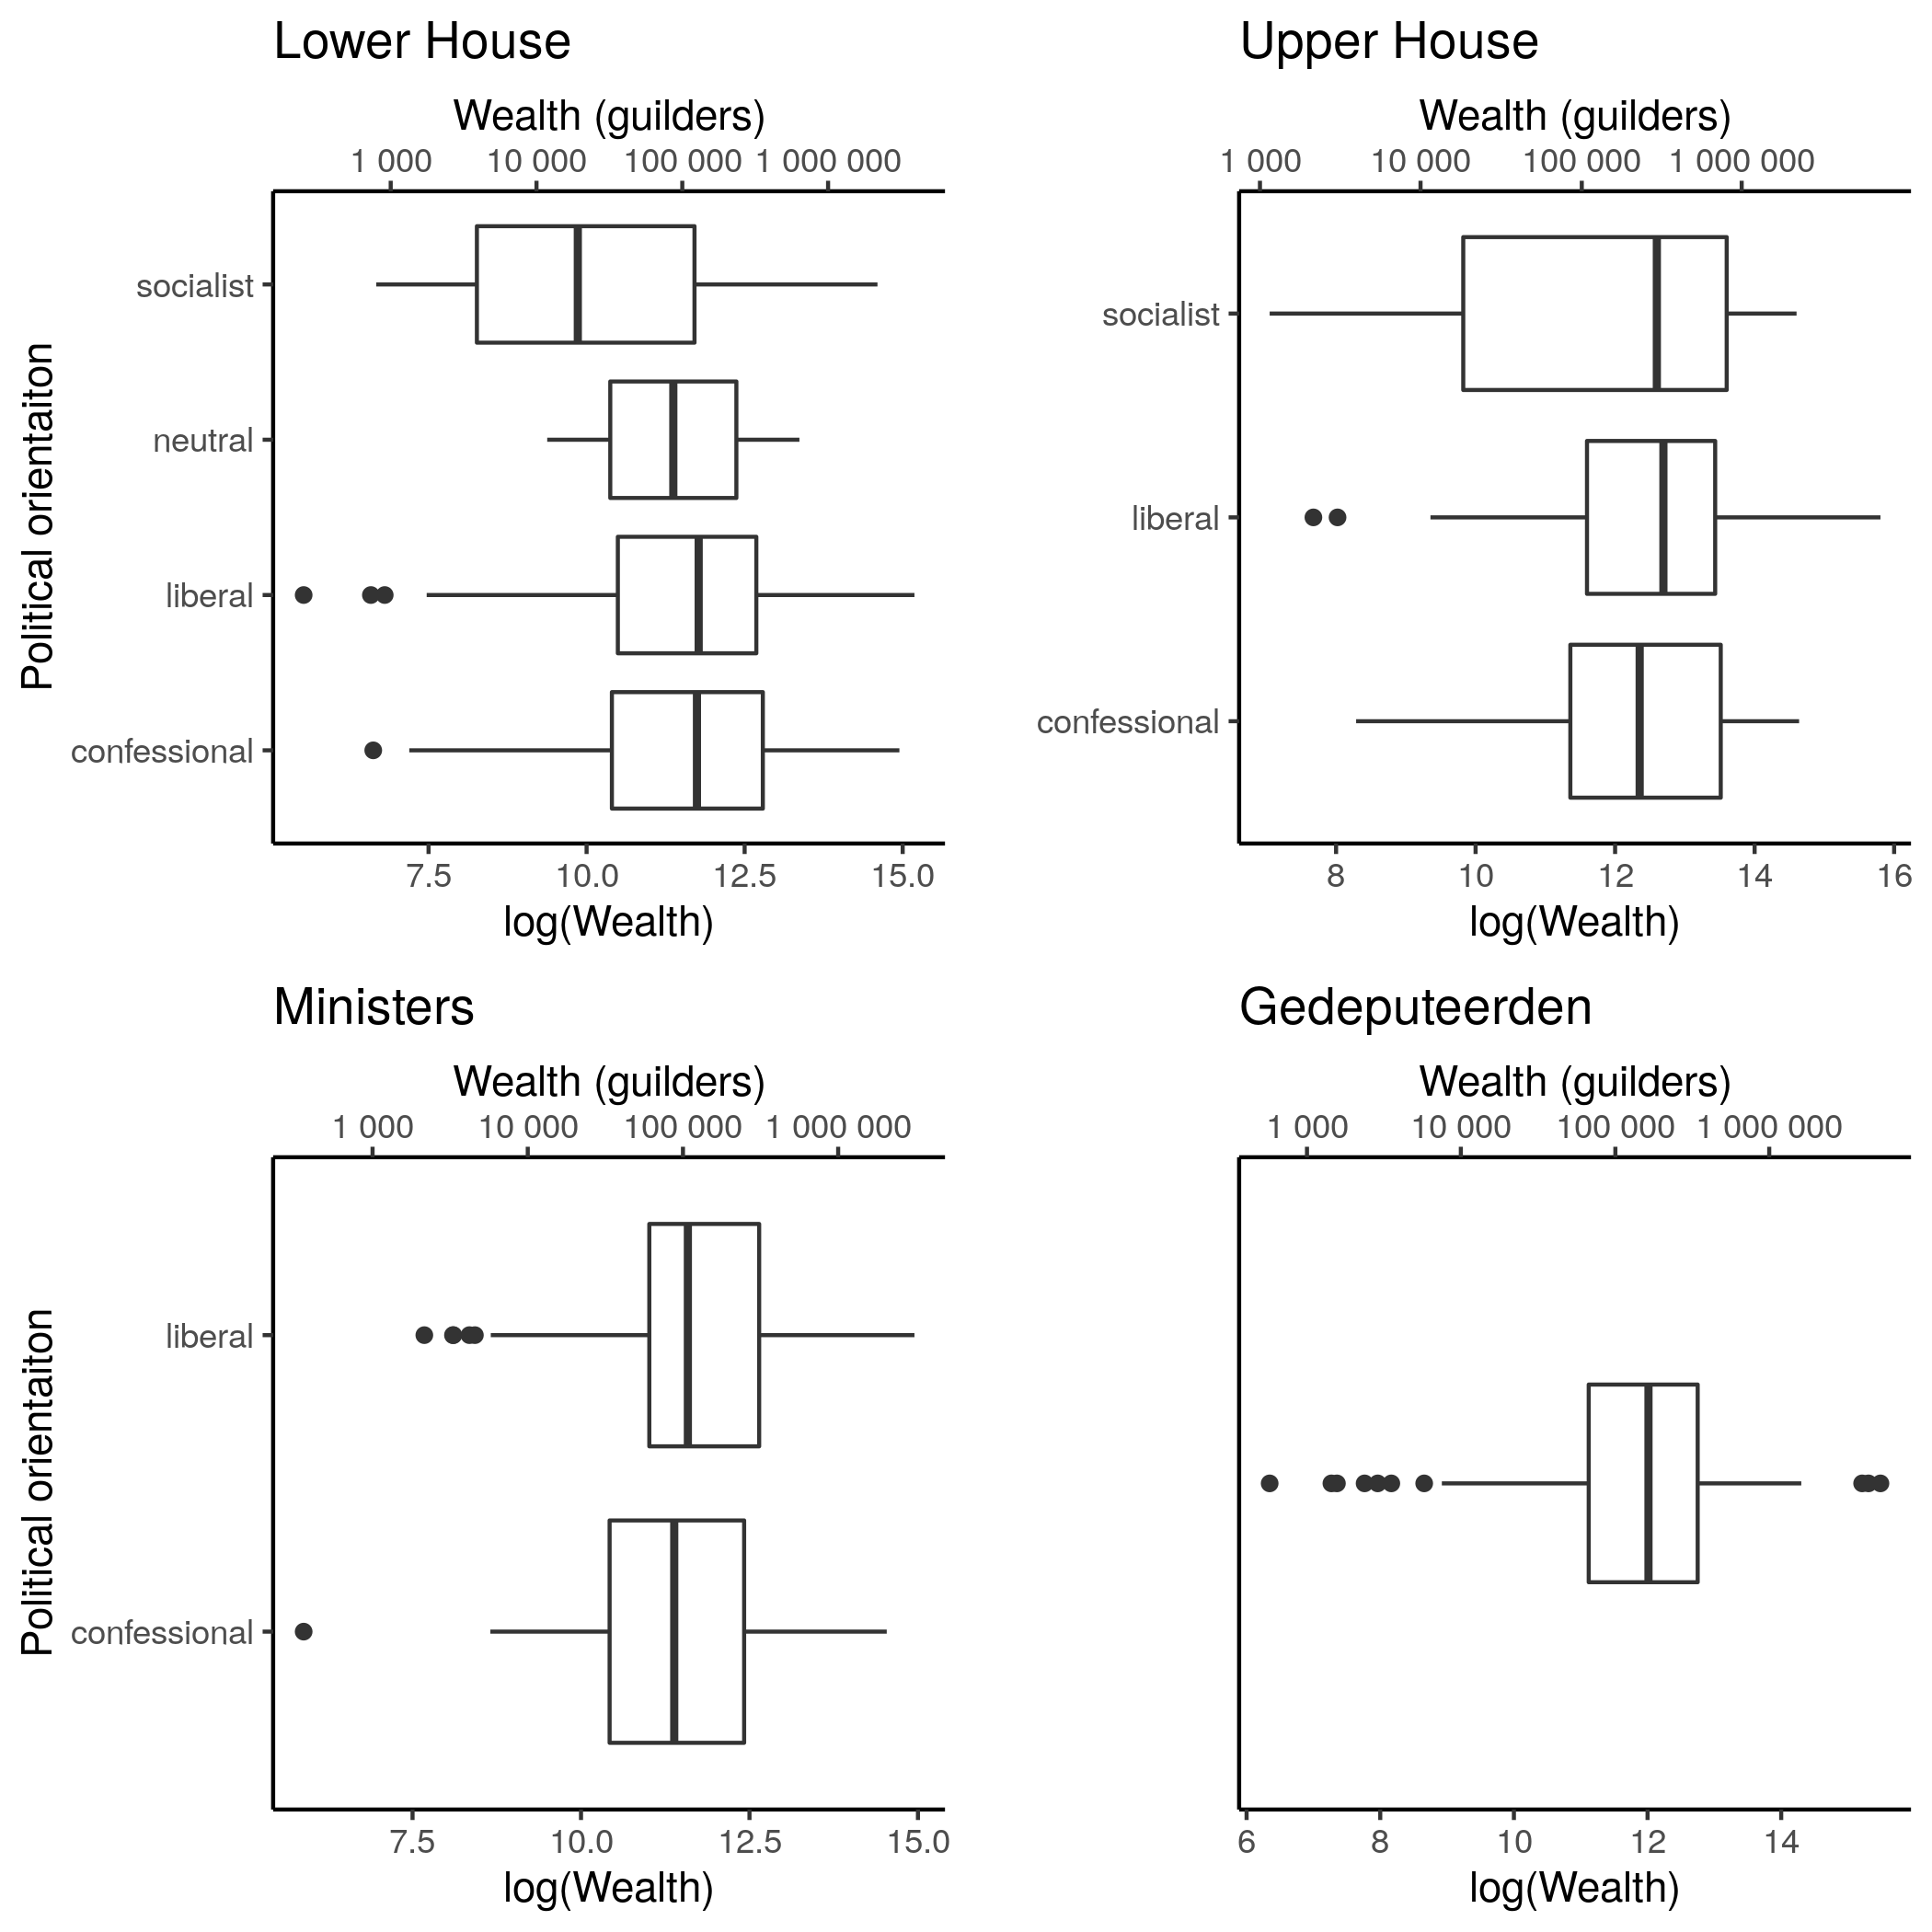
\includegraphics[scale = 0.80]{figures/fig_wealth_function.png}
%    \caption{Wealth Distribution According to Function and Party}
%    \label{fig:wealthfunction}
%\end{figure}

%\end{landscape}
%\clearpage

% Make table of fig_wealth_function
\begin{table}[!ht]
    \footnotesize
    \centering
    \begin{tabular}{llll}
        Year & House & Eligibility & Suffrage  \\ \hline
        1848 & Lower House & 30 yrs or older & Taxes (20-160 guilders) \\
        1848 & Upper House & Taxes paid (1/3000 inh) & Taxes (20-160 guilders) \\
        1887 & Lower House & 30 years or older & Taxes, home ownership, rents \\
        1887 & Upper House & Taxes paid (1/1500 inh) & Taxes, home ownership, rents \\
        1896 & Lower House & 30 years or older & Taxes, rents, wages, savings, exam \\
        1896 & Upper House & Taxes paid (1/1500 inh) & Taxes, rents, wages, savings, exam \\
        1917 & Lower House & Male, 25 years or older & Male, 23 years and older \\
        1917 & Upper House & Male, 25 years or older  & Male, 23 years and older \\
        1919 & Lower House & 25 years or older & 23 years and older \\
        1919 & Upper House & 25 years or older & 23 years and older \\ \hline
    \end{tabular}
    \caption{Changes in electoral laws}
    \label{tab:upperhouselowerhouse}
\end{table}
\clearpage

% latex table generated in R 4.0.2 by xtable 1.8-4 package
% Sun Oct  4 20:31:02 2020
\begin{table}[ht]
\centering
\begin{tabular}{lrrrrrr}
   
\multicolumn{7}{l}{Panel A: Lower House}\\ 
\hline
Political Affiliation & Mean & Median & StdDev & p25 & p75 & n \\\hline

confessional & 264.0 & 96.1 & 441.3 & 17.8 & 326.9 & 165 \\ 
  liberal & 328.1 & 104.2 & 629.1 & 19.5 & 302.8 & 146 \\ 
  neutral & 325.1 & 325.1 & 443.0 & 168.4 & 481.7 & 2 \\ 
  socialist & 201.1 & 13.1 & 496.9 & 3.0 & 112.0 & 23 \\ 
   \hline\\ 
\multicolumn{7}{l}{Panel B: Upper House}\\ 
\hline
Political Affiliation & Mean & Median & StdDev & p25 & p75 & n \\\hline
confessional & 471.6 & 214.4 & 577.3 & 69.1 & 696.7 & 78 \\ 
  liberal & 640.7 & 321.2 & 1052.3 & 99.3 & 681.6 & 82 \\ 
  socialist & 830.3 & 296.0 & 1190.0 & 148.6 & 1244.9 & 3 \\ 
   \hline\\ 
\multicolumn{7}{l}{Panel C: Ministers}\\ 
\hline
Political Affiliation & Mean & Median & StdDev & p25 & p75 & n \\\hline
confessional & 195.8 & 71.7 & 329.1 & 21.2 & 219.1 & 62 \\ 
  liberal & 254.8 & 105.6 & 452.0 & 45.8 & 298.6 & 63 \\ 
  neutral & 26.7 & 24.5 & 23.7 & 8.8 & 42.5 & 7 \\ 
  socialist & 106.6 & 58.3 & 103.7 & 51.9 & 113.0 & 4 \\ 
   \hline\\ 
\multicolumn{7}{l}{Panel D: Regional Executives}\\ 
\hline
Political Affiliation & Mean & Median & StdDev & p25 & p75 & n \\\hline
- & 348.8 & 154.4 & 688.3 & 54.1 & 331.9 & 157 \\ 
   \hline
\multicolumn{7}{l}{}\\
\end{tabular}
\caption{Wealth according to political affiliation ($\cdot 10^{3}$ guilders)} 
\label{tab:wealthfunction}
\end{table}
\clearpage

% latex table generated in R 4.0.2 by xtable 1.8-4 package
% Sun Oct  4 20:43:17 2020
\begin{table}[ht]
\centering
\begin{tabular}{lrrrrr}
   
\multicolumn{6}{l}{Panel A: Lower House}\\ 
\hline
Political Affiliation & Mean & Median & p25 & p75 & n \\\hline

confessional & 0.955 & 0.847 & 0.213 & 0.966 & 165 \\ 
  liberal & 0.966 & 0.860 & 0.277 & 0.964 & 146 \\ 
  neutral & 0.966 & 0.966 & 0.921 & 0.981 & 2 \\ 
  socialist & 0.939 & 0.162 & 0.000 & 0.869 & 23 \\ 
   \hline\\ 
\multicolumn{6}{l}{Panel B: Upper House}\\ 
\hline
Political Affiliation & Mean & Median & p25 & p75 & n \\\hline
confessional & 0.980 & 0.942 & 0.776 & 0.989 & 78 \\ 
  liberal & 0.987 & 0.966 & 0.854 & 0.989 & 82 \\ 
  socialist & 0.992 & 0.963 & 0.909 & 0.996 & 3 \\ 
   \hline\\ 
\multicolumn{6}{l}{Panel C: Ministers}\\ 
\hline
Political Affiliation & Mean & Median & p25 & p75 & n \\\hline
confessional & 0.936 & 0.787 & 0.319 & 0.943 & 62 \\ 
  liberal & 0.952 & 0.862 & 0.664 & 0.963 & 63 \\ 
  neutral & 0.437 & 0.388 & 0.000 & 0.640 & 7 \\ 
  socialist & 0.863 & 0.731 & 0.704 & 0.870 & 4 \\ 
   \hline\\ 
\multicolumn{6}{l}{Panel D: Regional Executives}\\ 
\hline
Political Affiliation & Mean & Median & p25 & p75 & n \\\hline
- & 0.968 & 0.913 & 0.714 & 0.967 & 157 \\ 
   \hline
\multicolumn{6}{l}{}\\
\end{tabular}
\caption{Estimates of the Place of Politicians in the Population Wealth Distribution} 
\label{tab:comp_population}
\end{table}
\clearpage

% latex table generated in R 4.0.2 by xtable 1.8-4 package
% Mon Oct  5 03:51:14 2020
\begin{table}[ht]
\centering
\begin{tabular}{lrrr}
   
\multicolumn{4}{l}{Panel A: Lower House}\\ 
\hline
harnas & Mean & Median & SD \\\hline

$>$ 2 Year & 283545 & 95326 & 502659 \\ 
  $<$ 2 Year & 278731 & 84325 & 491440 \\ 
   \hline\\ 
\multicolumn{4}{l}{Panel B: Upper House}\\ 
\hline
harnas & Mean & Median & SD \\\hline
$>$ 2 Year & 552511 & 291070 & 887025 \\ 
  $<$ 2 Year & 557900 & 281424 & 774221 \\ 
   \hline\\ 
\multicolumn{4}{l}{Panel C: Ministers}\\ 
\hline
harnas & Mean & Median & SD \\\hline
$>$ 2 Year & 296196 & 87861 & 957257 \\ 
  $<$ 2 Year & 71026 & 29174 & 145775 \\ 
   \hline\\ 
\multicolumn{4}{l}{Panel D: Regional Executives}\\ 
\hline
harnas & Mean & Median & SD \\\hline
$>$ 2 Year & 452183 & 232022 & 881262 \\ 
  $<$ 2 Year & 234235 & 100304 & 354270 \\ 
   \hline
\multicolumn{4}{l}{}\\
\end{tabular}
\caption{Wealth according to having died shortly after leaving office} 
\label{tab:harnas}
\end{table}
\clearpage

\begin{landscape}

\begin{figure}
    \centering
    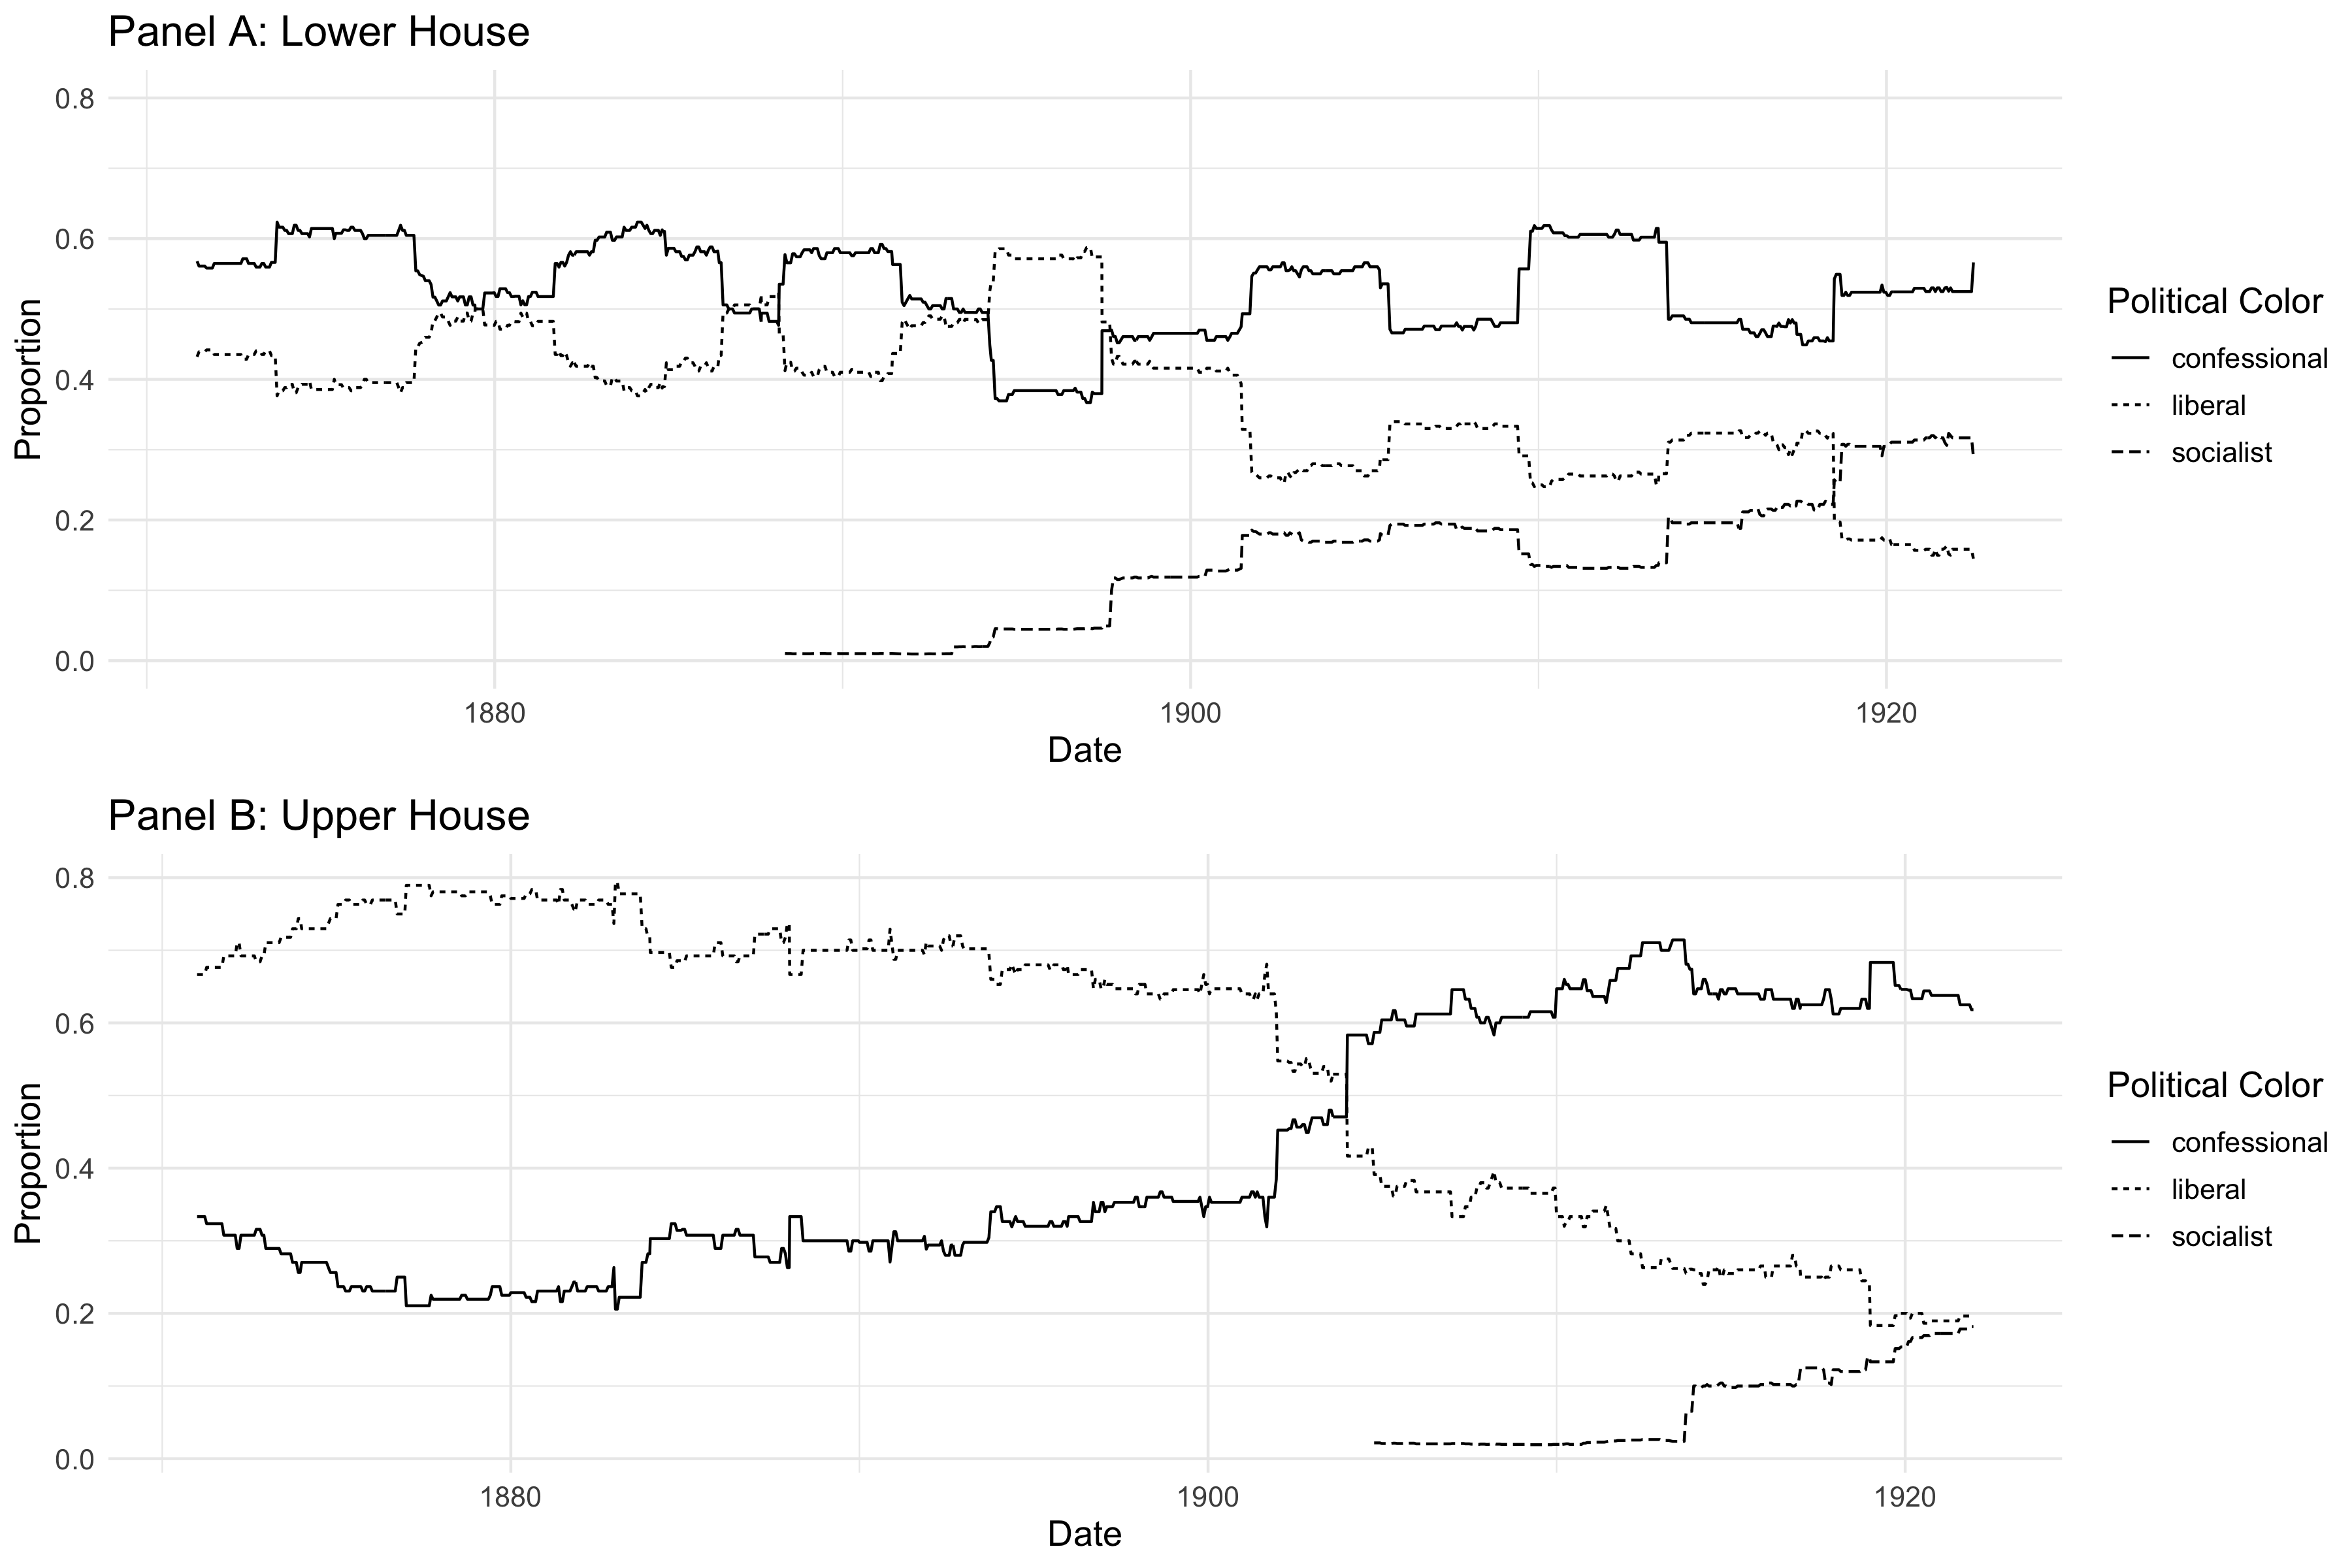
\includegraphics[scale=0.80]{figures/step4comp.png}
    \caption{Political Color of Parliament over Time}
    \label{fig:parltime}
\end{figure}

\end{landscape}
\clearpage

\begin{figure}
    \centering
    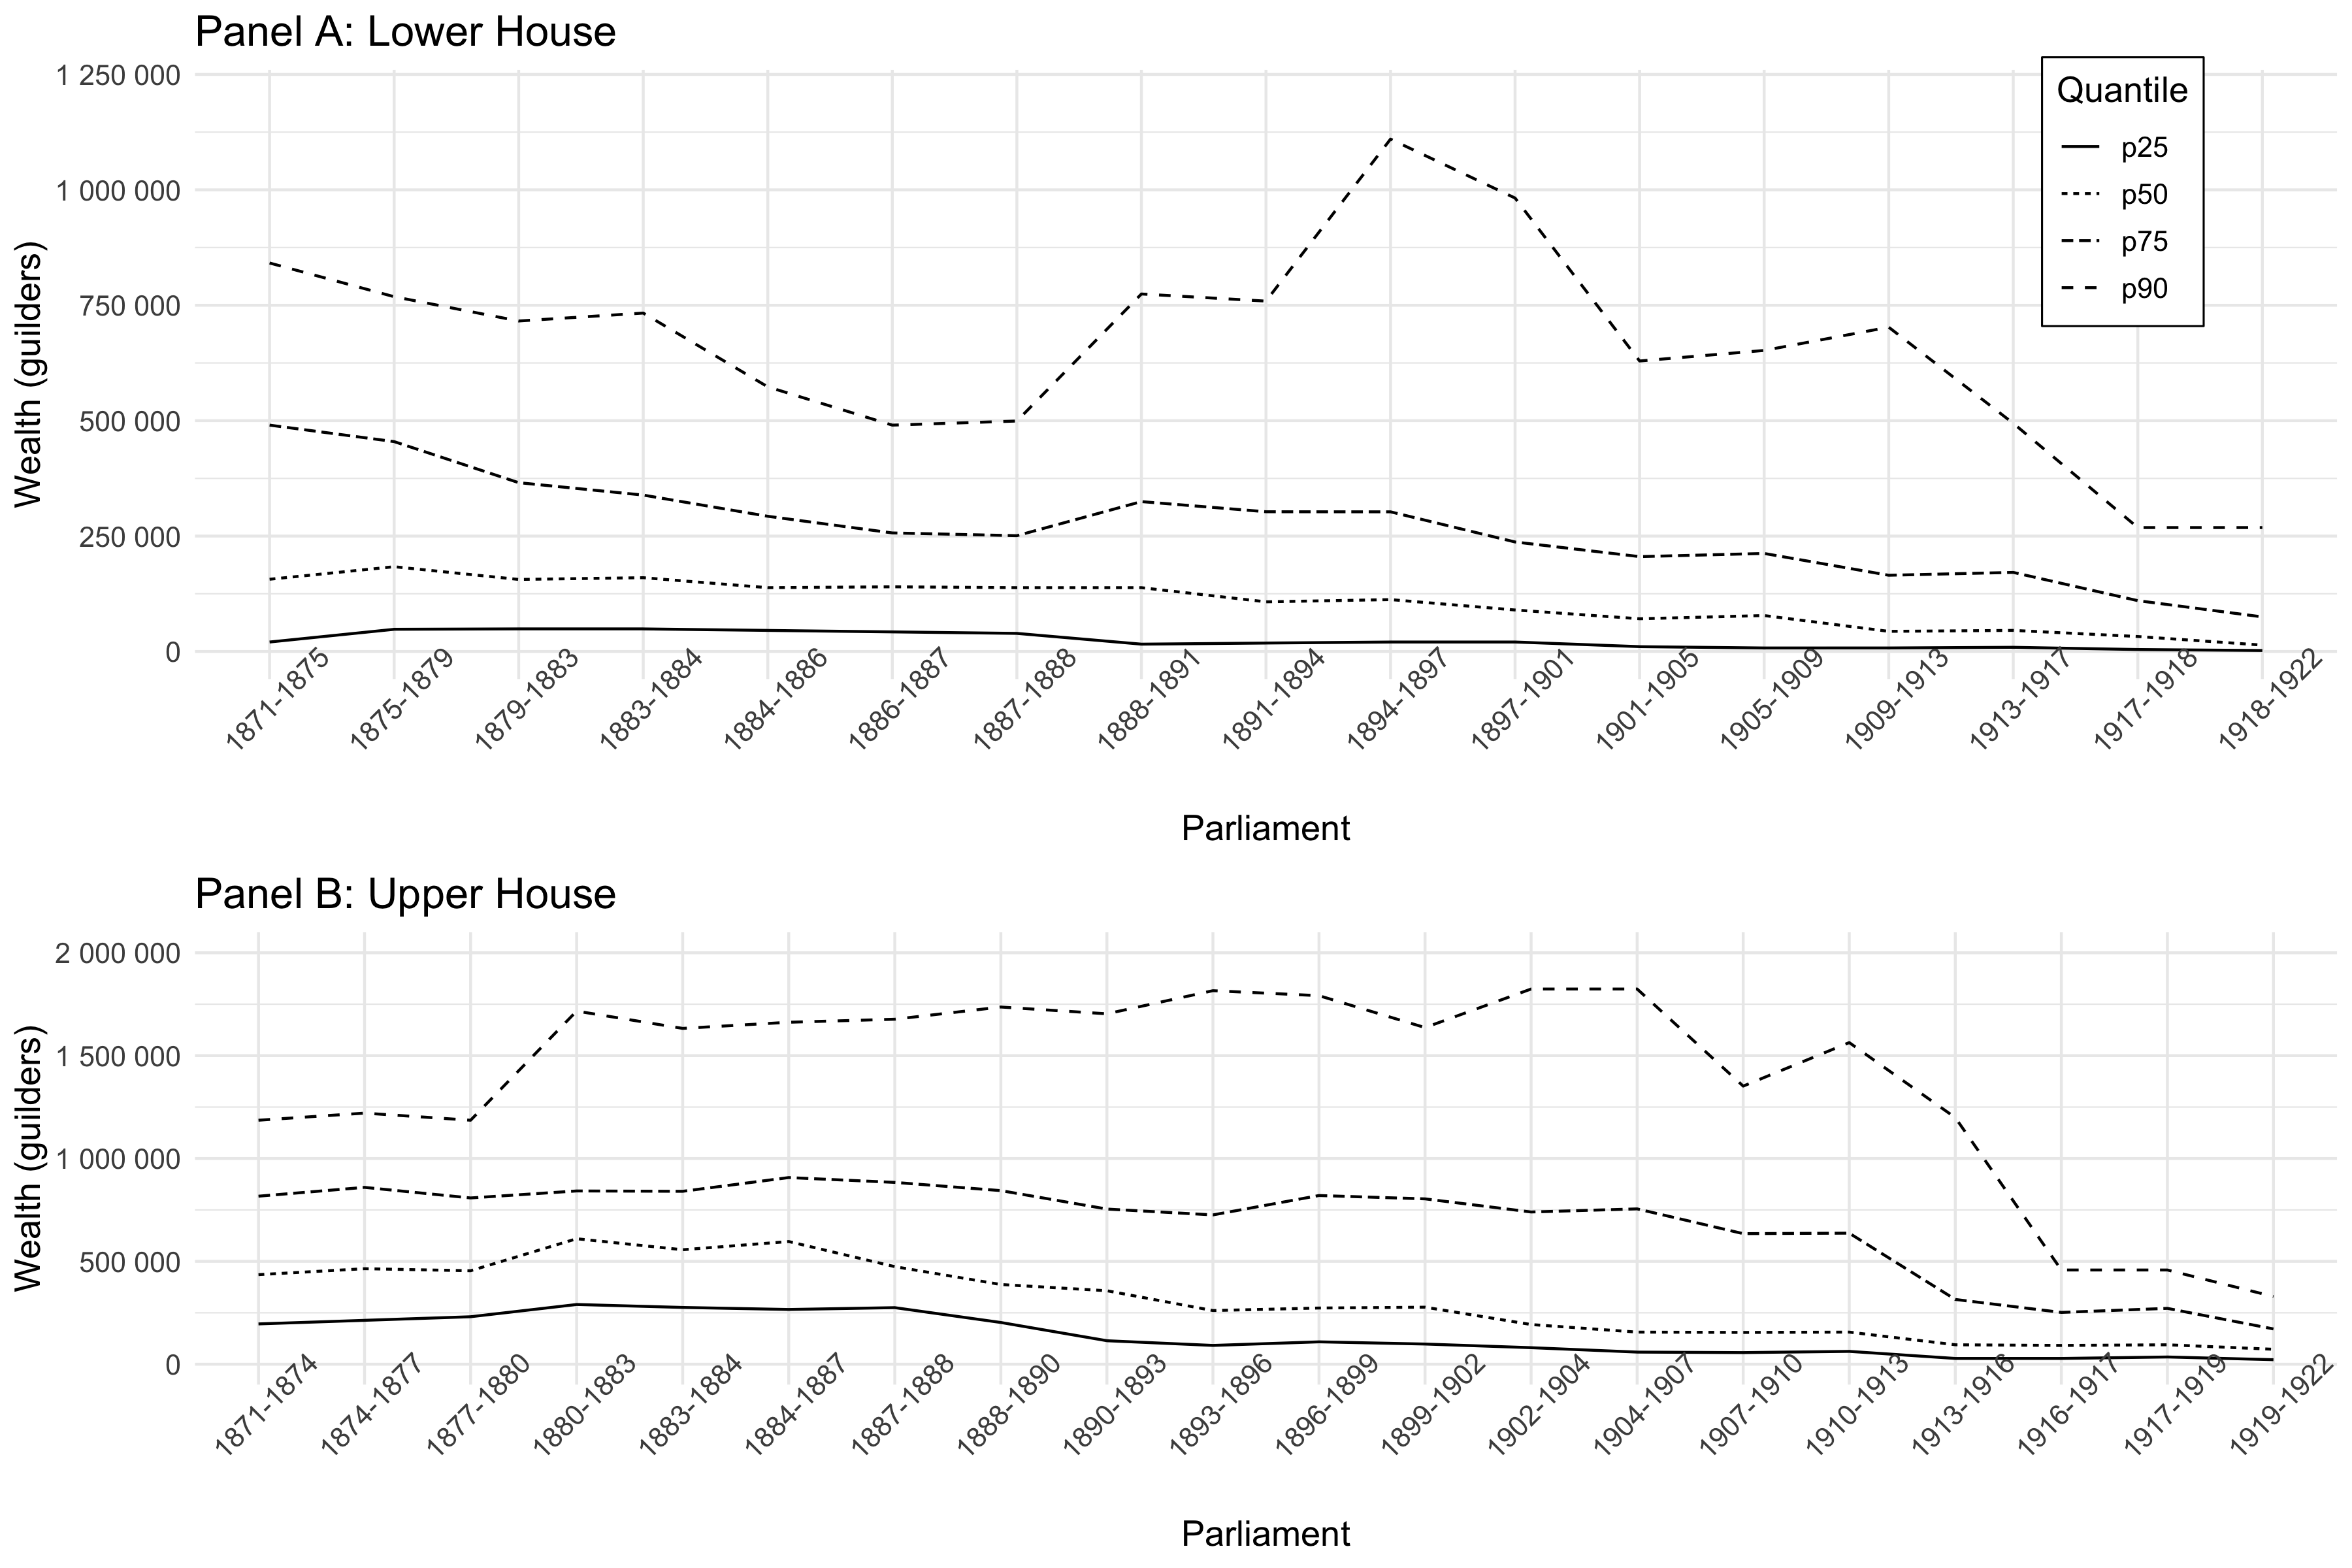
\includegraphics[scale=0.8]{figures/step5fig2wealthperparl.png}
    \caption{Wealth Distribution in Upper and Lower House over Time}
    \label{fig:avgwealthtime}
\end{figure}
\clearpage

\begin{figure}
    \centering
    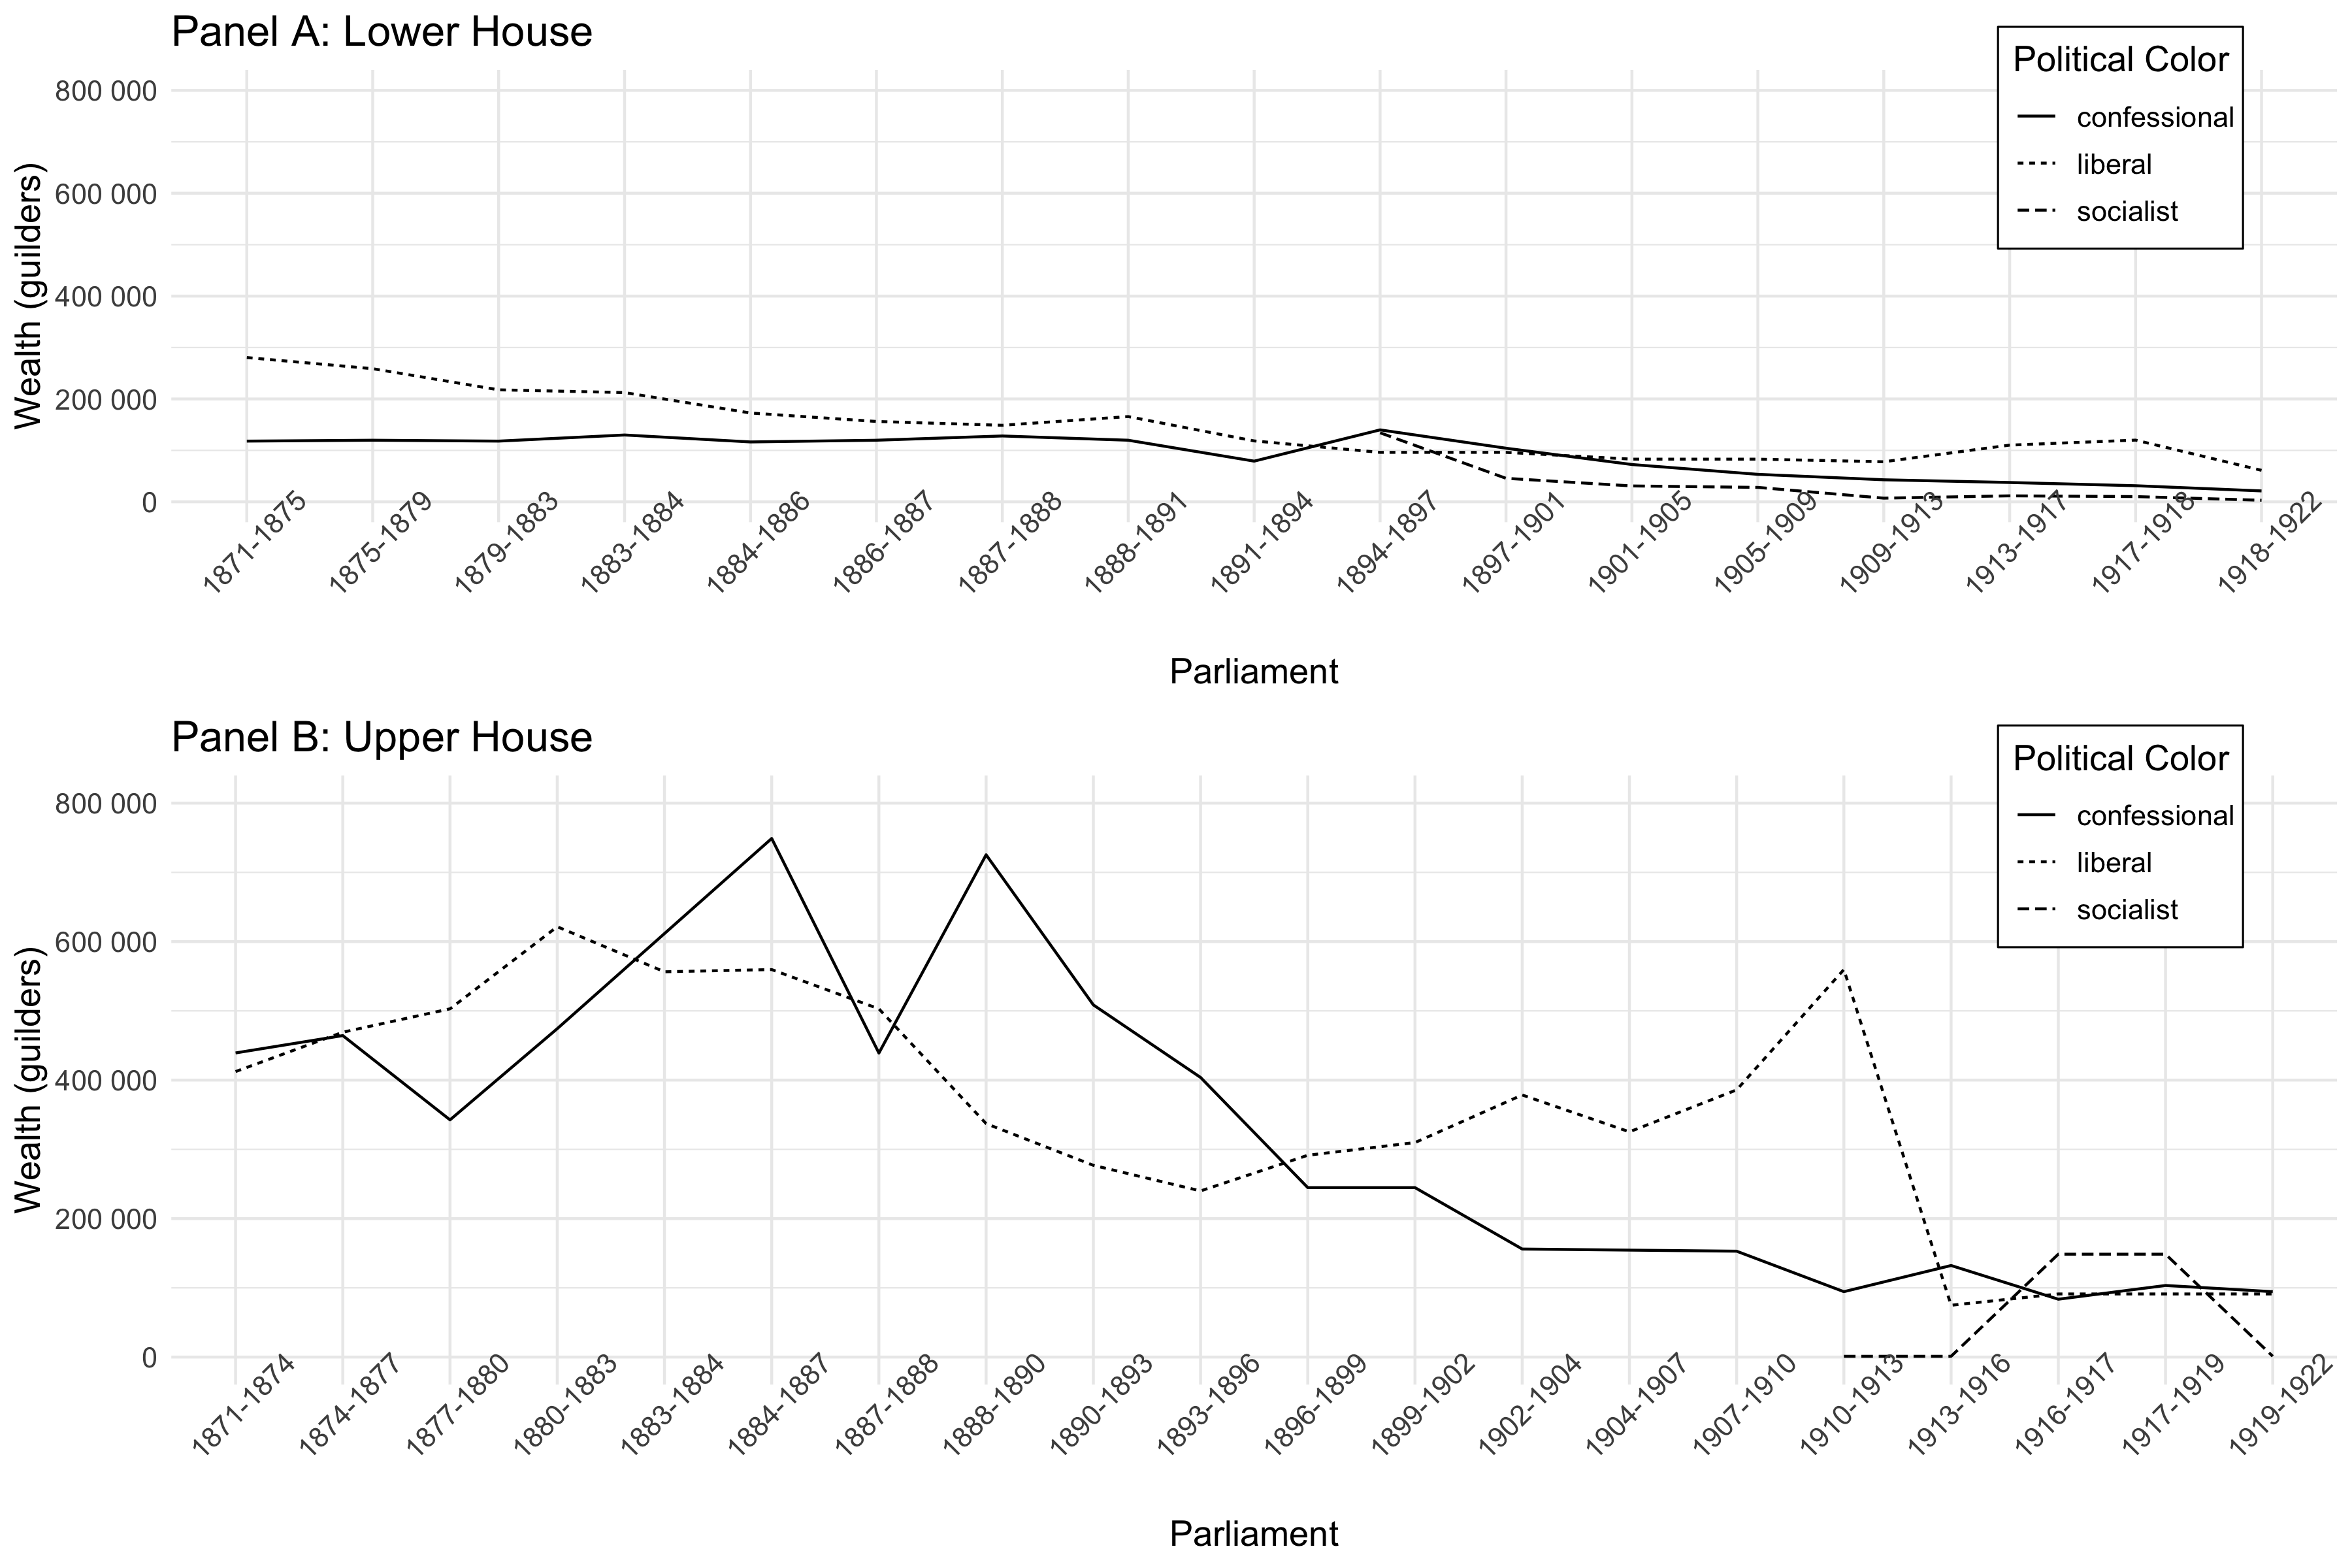
\includegraphics[scale=0.60]{figures/step8fig2wealthperparlperparty.png}
    \caption{Average Wealth per Parliament per Party}
    \label{fig:avgwealthtimeparty}
\end{figure}
\clearpage

\begin{landscape}
\begin{figure}
    \centering
    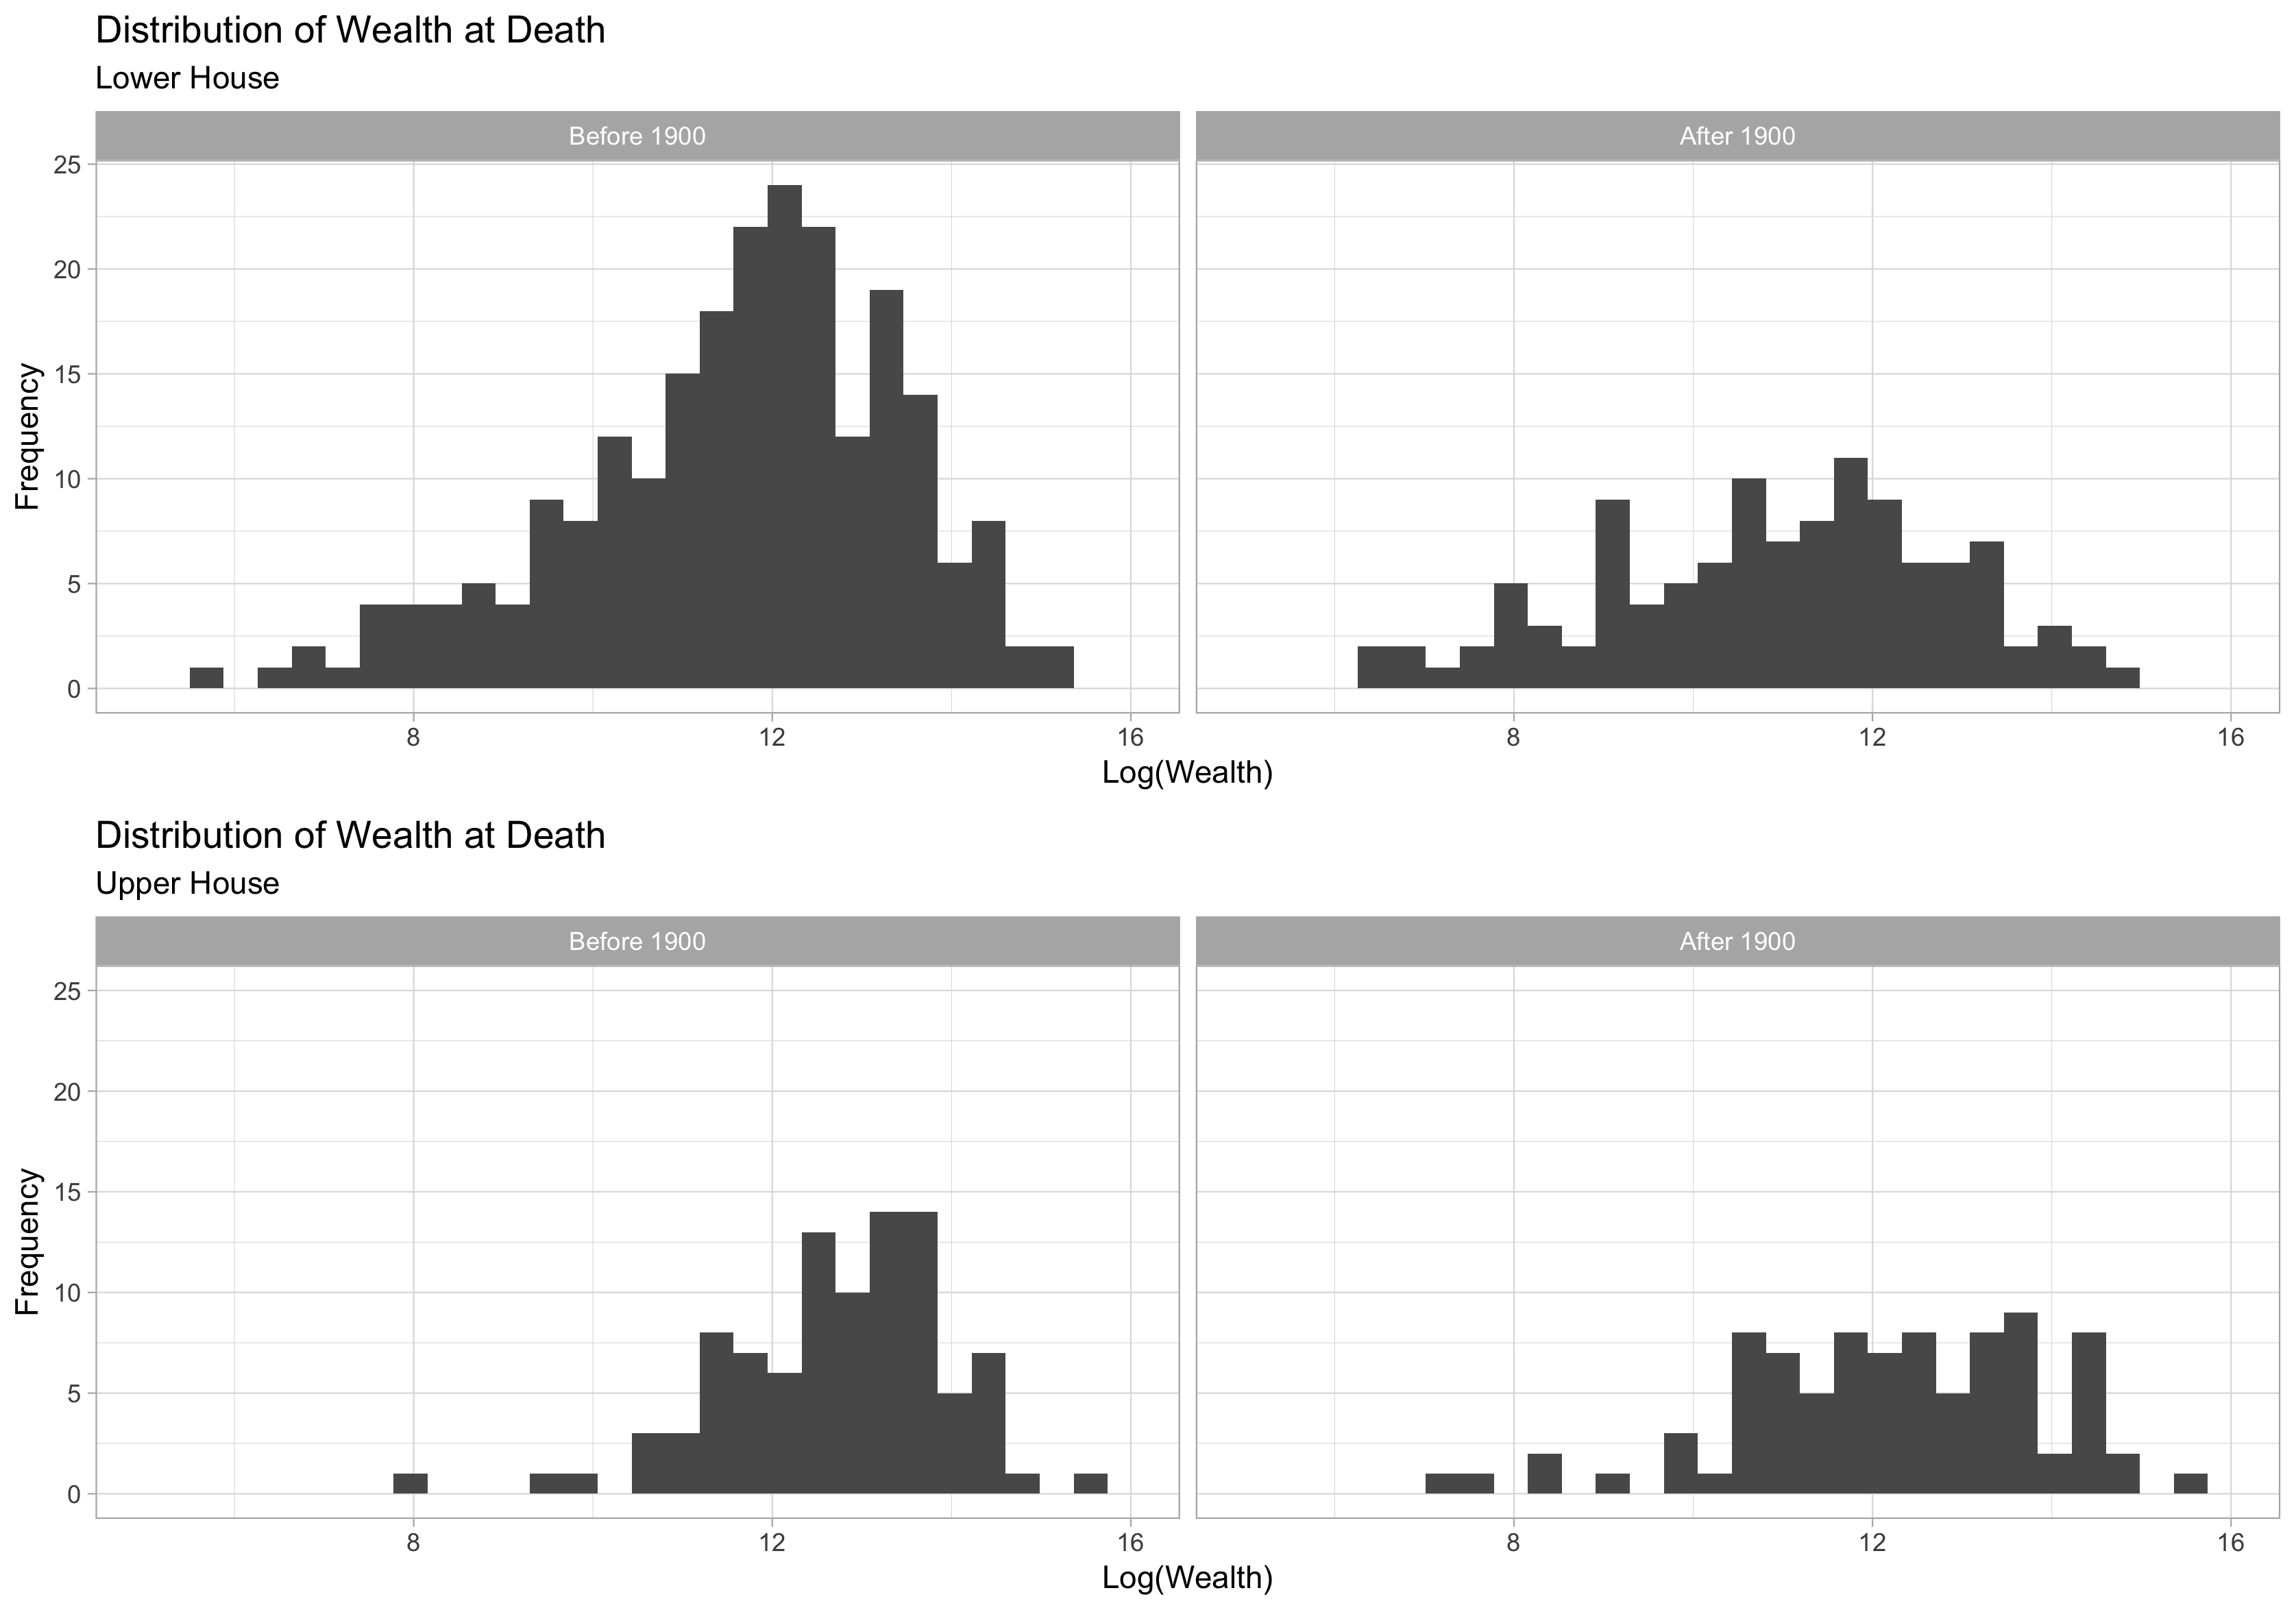
\includegraphics[scale=0.15]{figures/Histogram_wealth_per_parl.png}
    \caption{Wealth Distribution Before and After 1900 By House}
    \label{fig:histogram}
\end{figure}
\end{landscape}
\clearpage

% latex table generated in R 3.6.0 by xtable 1.8-4 package
% Mon Aug 31 14:10:07 2020
\begin{table}[ht]
\centering
\begin{tabular}{llllr}

\multicolumn{5}{l}{Panel A: Lower House}\\
\hline
Name & Begin & End & Death & Wealth \\\hline

George Hermann Hintzen & 1888 & 1897 & 1932 & 3,938.4 \\
  Carel Jan Emilius van Bylandt & 1894 & 1901 & 1902 & 3,840.4 \\
  Willem van Heeckeren van Kell & 1882 & 1884 & 1914 & 3,103.7 \\
  Willem Jan Roijaards van den Ham & 1888 & 1897 & 1897 & 2,918.3 \\
  Henri François Rudolf Hubrecht & 1901 & 1918 & 1926 & 2,221.3 \\
   \hline\\
\multicolumn{5}{l}{Panel B: Upper House}\\
\hline
Name & Begin & End & Death & Wealth \\\hline
Gerrit Jan van Heek & 1895 & 1903 & 1915 & 7,303.5 \\
  Dirk Laan & 1897 & 1905 & 1905 & 4,749.5 \\
  Cornelis Jacob Arnold den Tex & 1875 & 1882 & 1882 & 3,067.1 \\
  Jan Evert Scholten & 1902 & 1910 & 1918 & 2,364.5 \\
  Jan van der Lande & 1913 & 1932 & 1943 & 2,275.6 \\
   \hline\\
\multicolumn{5}{l}{Panel C: Ministers}\\
\hline
Name & Begin & End & Death & Wealth \\\hline
Willem Heeckeren van Kell & 1877 & 1879 & 1914 & 3,103.7 \\
  Robert Melvil baron van Lynden & 1901 & 1905 & 1910 & 2,057.1 \\
  Johannes Pieter Roetert Tak van Poortvliet & 1877 & 1894 & 1904 & 1,529.8 \\
  James Loudon & 1861 & 1862 & 1900 & 861.5 \\
  Daniël Théodore Gevers van Endegeest & 1856 & 1858 & 1877 & 833.8 \\
   \hline\\
\multicolumn{5}{l}{Panel D: Provincial Executives}\\
\hline
Name & Begin & End & Death & Wealth \\\hline
H. Royaards & 1873 & 1896 & 1898 & 5,310.2 \\
  D. Weel & 1888 & 1901 & 1911 & 4,440.3 \\
  H.A. Steengracht van Duivenvoorde & 1873 & 1880 & 1912 & 4,035.8 \\
  W. Heeckeren van Kell & 1877 & 1884 & 1914 & 3,103.7 \\
  H.F.R. Hubrecht & 1901 & 1918 & 1926 & 2,221.3 \\
   \hline
\multicolumn{5}{l}{}\\
\end{tabular}
\caption{5 Richest Politicians in each Function (1000 guilders)}
\label{tab:richestpols}
\end{table}

\clearpage


% latex table generated in R 3.6.3 by xtable 1.8-4 package
% Wed Aug 19 19:10:42 2020
\begin{table}[ht]
\centering
\begin{tabular}{lrrrrr}
  \hline
House & mean\_re & mean\_shares & mean\_bonds & mean\_misc & n \\ 
  \hline
Lower House & 0.28 & 0.19 & 0.40 & 0.13 & 245 \\ 
  Upper House & 0.44 & 0.19 & 0.30 & 0.07 &  99 \\ 
  Ministers & 0.20 & 0.20 & 0.47 & 0.13 &  96 \\ 
  Provincial Executives & 0.40 & 0.13 & 0.39 & 0.08 & 109 \\ 
   \hline
\end{tabular}
\caption{Before 1900} 
\label{fig:portcomp1_1}
\end{table}


% latex table generated in R 3.6.3 by xtable 1.8-4 package
% Wed Aug 19 19:05:15 2020
\begin{table}[ht]
\centering
\begin{tabular}{lrrrrr}
  \hline
House & mean\_re & mean\_shares & mean\_bonds & mean\_misc & n \\ 
  \hline
Lower House & 0.28 & 0.29 & 0.34 & 0.09 &  73 \\ 
  Upper House & 0.22 & 0.28 & 0.40 & 0.10 &  55 \\ 
  Ministers & 0.14 & 0.33 & 0.39 & 0.14 &  38 \\ 
  Provincial Executives & 0.32 & 0.25 & 0.37 & 0.06 &  45 \\ 
   \hline
\end{tabular}
\caption{After 1900} 
\label{fig:portcomp1_2}
\end{table}


% latex table generated in R 3.6.3 by xtable 1.8-4 package
% Wed Aug 19 19:05:15 2020
\begin{table}[ht]
\centering
\begingroup\small
\begin{tabular}{llrrrrr}
  \hline
House & class & mean\_re & mean\_shares & mean\_bonds & mean\_misc & n \\ 
  \hline
Lower House & confessional & 0.32 & 0.19 & 0.35 & 0.14 & 160 \\ 
  Lower House & liberal & 0.23 & 0.24 & 0.43 & 0.10 & 134 \\ 
  Lower House & neutral & 0.66 & 0.09 & 0.25 & 0.01 &   2 \\ 
  Lower House & socialist & 0.22 & 0.21 & 0.41 & 0.16 &  22 \\ 
  Upper House & confessional & 0.35 & 0.19 & 0.34 & 0.11 &  72 \\ 
  Upper House & liberal & 0.37 & 0.25 & 0.33 & 0.05 &  79 \\ 
  Upper House & socialist & 0.52 & 0.10 & 0.29 & 0.09 &   3 \\ 
  Ministers & confessional & 0.24 & 0.20 & 0.42 & 0.14 &  61 \\ 
  Ministers & liberal & 0.14 & 0.26 & 0.48 & 0.13 &  63 \\ 
  Ministers & neutral & 0.10 & 0.24 & 0.53 & 0.13 &   6 \\ 
  Ministers & socialist & 0.21 & 0.36 & 0.38 & 0.06 &   4 \\ 
   \hline
\end{tabular}
\endgroup
\caption{Portfolio Composition according to Political Color} 
\label{fig:portcomp2}
\end{table}

\clearpage

\begin{landscape}
% latex table generated in R 3.6.3 by xtable 1.8-4 package
% Wed Aug 19 10:37:22 2020
\begin{table}[ht]
\centering
\begin{tabular}{lrrrrr}
  \hline
Government & Mean & Median & SD & N & WealthPM \\ 
  \hline
Thorbecke III & 178154 & 95554 & 201112 & 7 &  \\ 
  De Vries/Fransen van de Putte & 81432 & 60689 & 76062 & 7 &  \\ 
  Heemskerk/Van Lynden van Sandenburg & 291140 & 220192 & 280563 & 9 & 623456 \\ 
  Kappeyne van de Coppello & 723896 & 446626 & 942720 & 10 & 485686 \\ 
  Van Lynden van Sandenburg & 220697 & 160340 & 237914 & 10 & 748926 \\ 
  Heemskerk Azn. & 152602 & 57739 & 190782 & 13 & 623456 \\ 
  Mackay & 92411 & 81022 & 88781 & 8 & 246825 \\ 
  Van Tienhoven & 406770 & 233273 & 568110 & 6 & 365691 \\ 
  Röell & 158083 & 55433 & 207810 & 7 & 559626 \\ 
  Pierson & 98497 & 100291 & 55039 & 7 &  \\ 
  Kuyper & 317188 & 53429 & 770428 & 7 & 112404 \\ 
  De Meester & 156490 & 63356 & 244954 & 9 & 36111 \\ 
  Heemskerk & 62610 & 21440 & 108579 & 10 &  \\ 
  Cort van der Linden & 109307 & 97571 & 66149 & 8 & 100291 \\ 
  Ruijs de Beerenbrouck I & 80876 & 24459 & 145993 & 7 &  \\ 
   \hline
\end{tabular}
\caption{Average Wealth of Governments} 
\end{table}

\clearpage


\begin{figure}
    \centering
    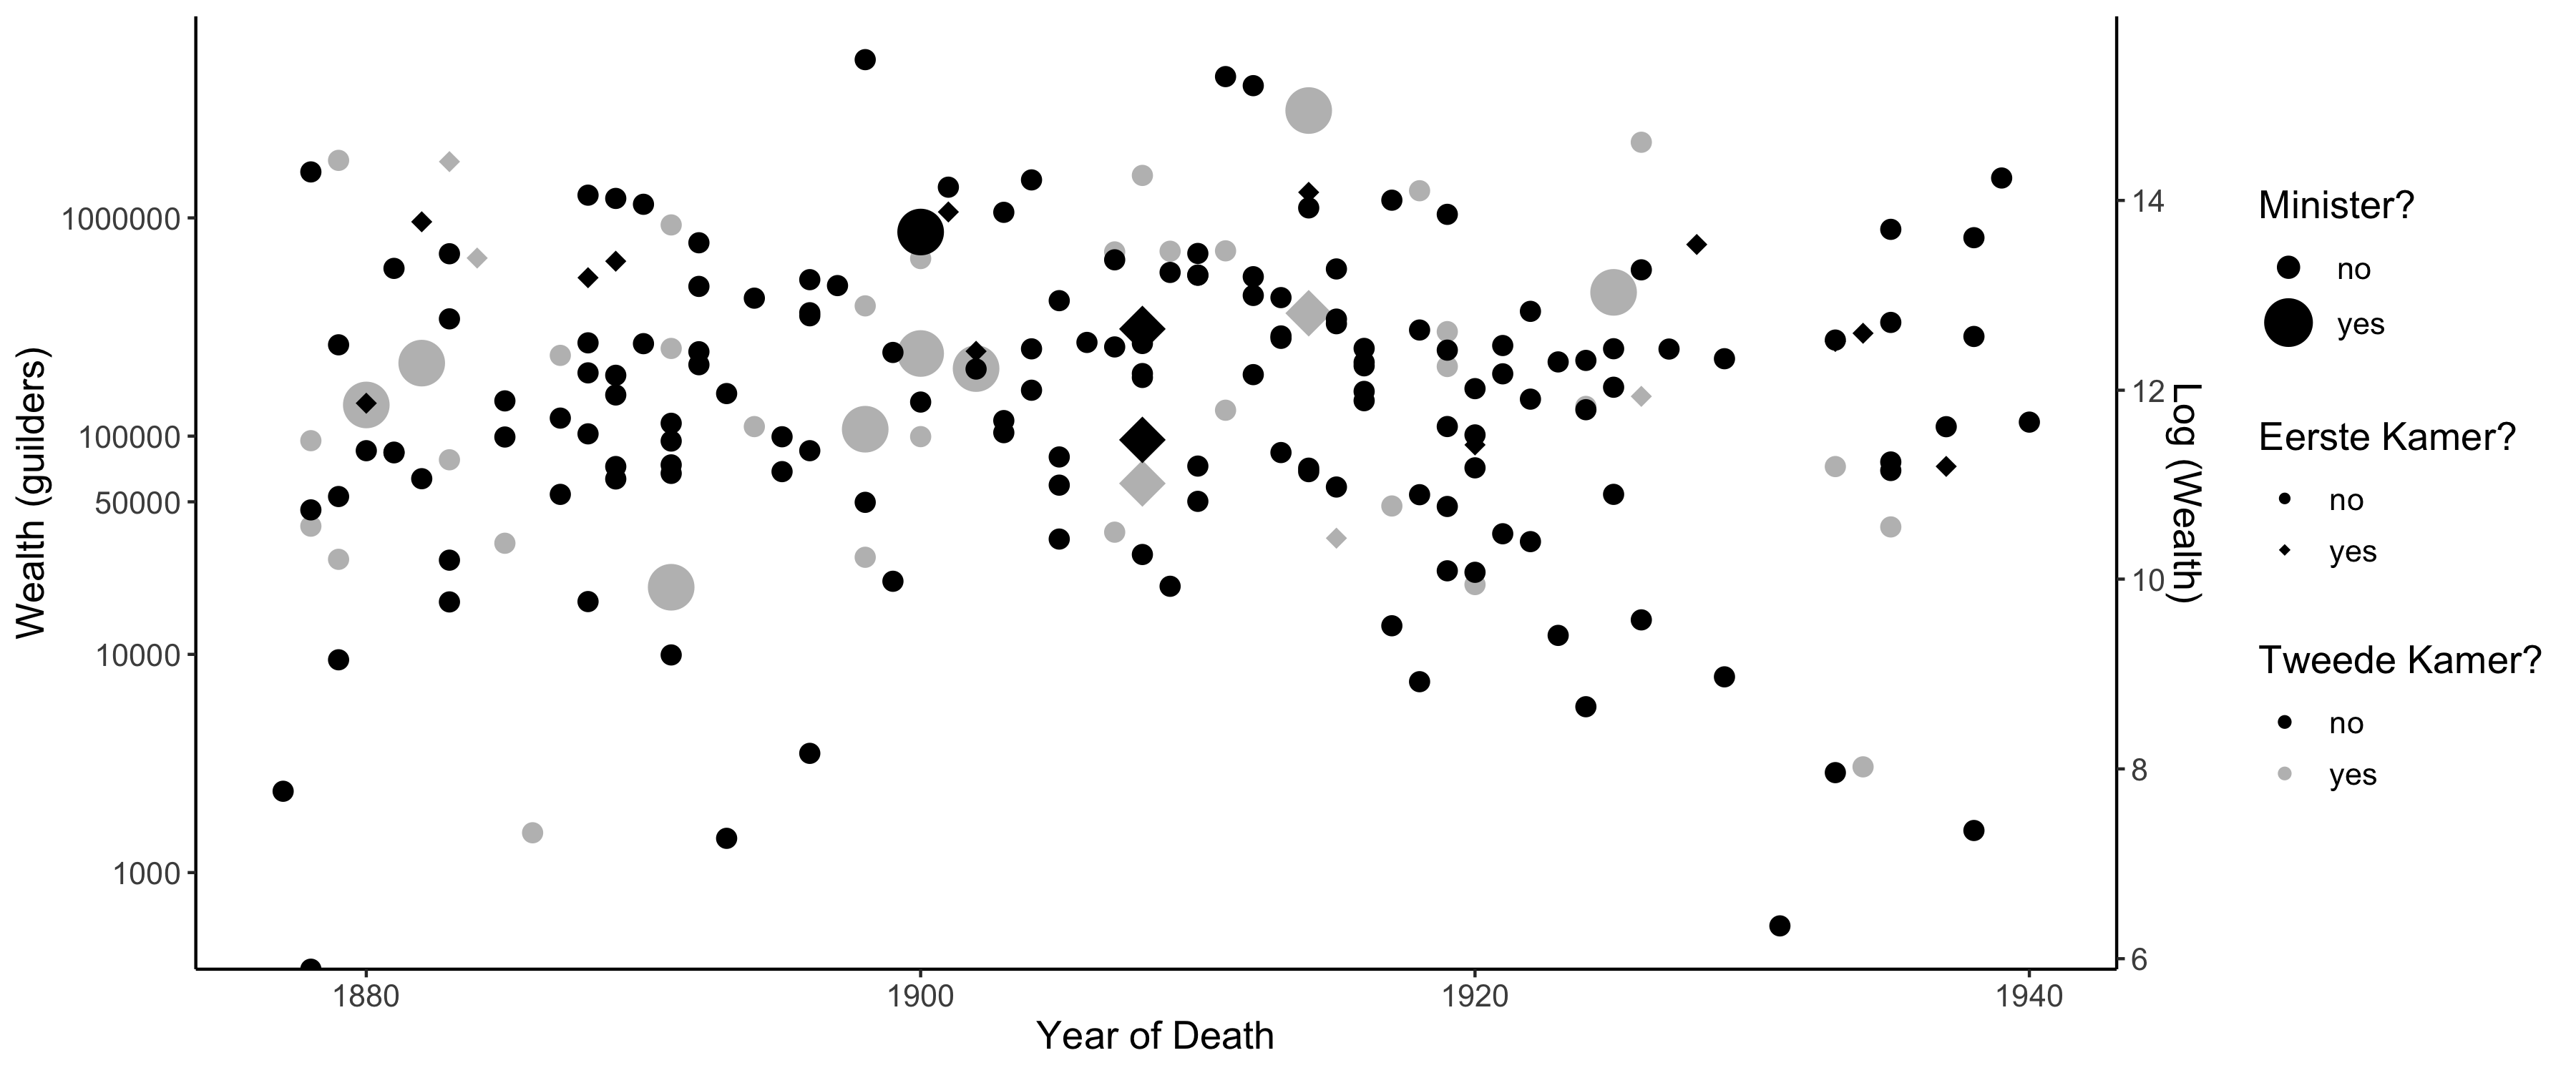
\includegraphics[scale = 0.17]{figures/wealth_dep.png}
    \caption{Wealth of Provincial Executives over Time}
    \label{fig:avgwealthprovexec}
\end{figure}
\clearpage
\end{landscape}

% latex table generated in R 4.0.2 by xtable 1.8-4 package
% Mon Oct  5 02:26:50 2020
\begin{table}[ht]
\centering
\begingroup\footnotesize
\begin{tabular}{lrrrrrr}
   
\multicolumn{7}{l}{Panel A:Lower House}\\ 
\hline
parliament & min & p25 & p75 & max & gini & gini2 \\\hline

1871-1875 & 1.33 & 28.7 & 521.8 & 1834.6 & 0.606 & 0.598 \\ 
  1875-1879 & 1.33 & 61.8 & 469.7 & 1834.6 & 0.589 & 0.571 \\ 
  1879-1883 & 1.33 & 63.5 & 424.9 & 3103.7 & 0.602 & 0.572 \\ 
  1883-1884 & 1.33 & 65.2 & 413.8 & 3103.7 & 0.596 & 0.557 \\ 
  1884-1886 & 0.90 & 65.5 & 307.6 & 1178.6 & 0.528 & 0.514 \\ 
  1886-1887 & 0.90 & 84.3 & 269.9 & 1331.8 & 0.523 & 0.499 \\ 
  1887-1888 & 0.90 & 79.9 & 270.1 & 1565.3 & 0.542 & 0.512 \\ 
  1888-1891 & 0.75 & 58.8 & 393.7 & 3938.4 & 0.655 & 0.621 \\ 
  1891-1894 & 0.75 & 35.0 & 324.1 & 3938.4 & 0.692 & 0.661 \\ 
  1894-1897 & 0.75 & 34.1 & 302.9 & 3938.4 & 0.741 & 0.719 \\ 
  1897-1901 & 0.25 & 23.5 & 287.6 & 3938.4 & 0.755 & 0.736 \\ 
  1901-1905 & 0.73 & 23.5 & 277.2 & 2221.3 & 0.715 & 0.699 \\ 
  1905-1909 & 0.73 & 20.0 & 258.1 & 2221.3 & 0.721 & 0.715 \\ 
  1909-1913 & 0.73 & 15.1 & 181.6 & 2221.3 & 0.770 & 0.761 \\ 
  1913-1917 & 0.73 & 13.1 & 212.4 & 2221.3 & 0.725 & 0.691 \\ 
  1917-1918 & 0.73 & 9.8 & 133.2 & 2221.3 & 0.744 & 0.620 \\ 
  1918-1922 & 1.00 & 8.4 & 96.1 & 638.3 & 0.703 & 0.679 \\ 
   \hline\\ 
\multicolumn{7}{l}{Panel B:Upper House}\\ 
\hline
parliament & min & p25 & p75 & max & gini & gini2 \\\hline
1871-1874 & 3.04 & 244.6 & 821.1 & 1743.0 & 0.458 & 0.444 \\ 
  1874-1877 & 3.04 & 258.4 & 880.5 & 3067.1 & 0.487 & 0.445 \\ 
  1877-1880 & 11.53 & 272.1 & 812.5 & 3067.1 & 0.459 & 0.415 \\ 
  1880-1883 & 11.53 & 303.3 & 843.9 & 3067.1 & 0.445 & 0.410 \\ 
  1883-1884 & 11.53 & 281.4 & 842.2 & 1966.1 & 0.415 & 0.402 \\ 
  1884-1887 & 48.10 & 275.0 & 912.3 & 1966.1 & 0.418 & 0.409 \\ 
  1887-1888 & 48.10 & 276.9 & 903.0 & 2057.1 & 0.436 & 0.424 \\ 
  1888-1890 & 19.21 & 206.8 & 845.5 & 2057.1 & 0.499 & 0.493 \\ 
  1890-1893 & 19.21 & 123.0 & 789.8 & 2057.1 & 0.542 & 0.537 \\ 
  1893-1896 & 19.21 & 105.6 & 766.4 & 7303.5 & 0.654 & 0.574 \\ 
  1896-1899 & 39.49 & 122.8 & 832.8 & 7303.5 & 0.661 & 0.603 \\ 
  1899-1902 & 39.49 & 117.0 & 826.4 & 7303.5 & 0.656 & 0.596 \\ 
  1902-1904 & 4.53 & 90.9 & 743.7 & 7303.5 & 0.707 & 0.653 \\ 
  1904-1907 & 2.15 & 67.1 & 817.1 & 4749.5 & 0.680 & 0.646 \\ 
  1907-1910 & 2.15 & 68.2 & 641.7 & 2364.5 & 0.647 & 0.639 \\ 
  1910-1913 & 1.15 & 68.2 & 641.7 & 2364.5 & 0.654 & 0.647 \\ 
  1913-1916 & 1.15 & 33.4 & 335.4 & 2275.6 & 0.729 & 0.724 \\ 
  1916-1917 & 1.15 & 33.4 & 262.9 & 2193.8 & 0.731 & 0.692 \\ 
  1917-1919 & 1.15 & 39.1 & 277.7 & 2193.8 & 0.706 & 0.661 \\ 
  1919-1922 & 1.15 & 25.0 & 196.7 & 702.4 & 0.590 & 0.544 \\ 
   \hline
\multicolumn{7}{l}{}\\
\end{tabular}
\endgroup
\caption{Wealth Distribution over Time (1000 Guilders)} 
\label{tab:ginicoef}
\end{table}

\end{document}
